% !TeX spellcheck = cs_CZ
% Differential calculus
%{\tikzset{external/prefix={tikz/MAI/}}
% \tikzset{external/figure name/.add={ch03_}{}}
%---------------------------------------------------------------------------------------------------
% Limits_of_Functions.tex
%---------------------------------------------------------------------------------------------------
\setchaptertoc
\chapter{Funkce jedné proměnné}\label{mai:IchapIII}
  \small
  S funkcemi se setkáváme na každém kroku nejen ve fyzice a v ostatních přírodních vědách, ale i v
  každodenním životě. Každá situace, kdy jsou nějaký jev či veličina jednoznačně a nevyhnutelně
  určeny jinými jevy či veličinami, se dá popsat pomocí funkce\footnote{V matematice abstrahujeme
  při zkoumání funkcionálních závislostí od konkrétní fyzikální povahy proměnných veličin a chápeme
  je jako \uv{bezrozměrné veličiny}, tedy jako číselné proměnné. Někdy je jednoduché takovou} funkci
  sestavit. Snadno například můžeme zjistit, jakou dráhu urazí automobil jedoucí známou rychlostí v
  závislosti na tom, jak dlouho jede. Nebo dokážeme určit přírůstek našich úspor ve spořitelně v
  závislosti na době spoření, pokud známe úrokovou míru a její změny. Jindy je naopak skoro nemožné
  přijít na to, jak taková funkce vypadá, neboť nemáme dostatek informací o parametrech, které do
  jejího zápisu vstupují. Třeba takovou závislost teploty ovzduší v daném okamžiku na zeměpisné
  poloze a nadmořské výšce, kterou bychom si mohli představit jako jednu ze samozřejmých součástí
  předpovědi počasí, bychom asi nesestavili. Popis jevů pomocí funkcí je v každém případě velmi
  užitečný. Má však svá pravidla, s nimiž se v této kapitole seznámíme. Závisí-li zkoumaný jev nebo
  veličina na jediné veličině, jejíž hodnoty jsou reálné a buď se mění známým způsobem, nebo si je
  můžeme dokonce volit, hovoříme o \textbf{funkci jedné reálné proměnné}. A lze-li zkoumaný jev nebo
  veličinu kvantifikovat rovněž pomocí reálných hodnot, jedná se o \textbf{reálnou funkci jedné
  reálné proměnné}. Právě o takových funkcích bude v této kapitole řeč. V aplikacích se budeme
  věnovat především funkcím, které mají význam ve fyzice a v přírodních vědách. Velmi často půjde o
  funkce, kde reálnou proměnnou je čas. Jevy v přírodě podléhají totiž principu příčinnosti, a tak
  lze velké množství veličin popisujících přírodní jevy vyjádřit na základě znalosti přírodních
  zákonů jako funkce času. 
  \cite[s.~53]{Musilova2009MA1}
  \normalsize
  \section{Funkce a její graf}\label{mai:IchapIIIsecI}
    V tomto odstavci se naučíme funkce zadávat, počítat s nimi a vyjádřit je velmi přehledným 
    způsobem - jejich \emph{grafem}. Zopakujme, že každou \textbf{reálnou funkci}, jejíž 
    definiční obor je podmnožina množiny \(\realset\), nazýváme \textbf{reálnou funkcí jedné 
    reálné proměnné}\footnote{Místo názvu \uv{reálná funkce jedné reálné proměnné} budeme pro 
    stručnost používat pouze název \uv{funkce}, pokud nebude řečeno něco jiného}.
    
    Protože \emph{funkce je speciální případ zobrazení}, můžeme všech\-ny pojmy a obecné 
    vlastnosti zobrazení přenést i na funkce. Některé z nich však vzhledem k důležitosti 
    zopakujme, případně doplníme. Na druhé straně budeme studovat také ty vlastnosti, které jsou 
    specifické pro tento speciální druh zobrazení.
    
    \begin{note}
      Je-li \(\mathcal{D}_f = \naturalset\), jedná se o \textbf{posloupnost}. (Speciálním 
      případem reálných funkcí jedné reálné proměnné jsou \emph{posloupnosti reálných čísel)}.
    \end{note}
      
    \subsection{Způsoby zadání funkce}\label{mai:IchapIIIsecIssecI}
      Nejprve funkci definujeme. Předpokládejme, že reálná proměnná, na níž bude záviset náš jev, 
      má dovoleno nabývat hodnot z určité předem stanovené podmnožiny \(D\subseteq\realset\) 
      reálných čísel. Předpokládejme dále, že podle určitého pravidla, předpisu, dokážeme pro 
      \emph{každou hodnotu} \(x\) množiny \(\mathcal{D}_f\), tj. \(x \in \mathcal{D}_f\), určit 
      \emph{právě jednu} reálnou hodnotu \(y\). Každé hodnotě \(x \in D\) tedy nějaké \(y\) 
      příslušet \emph{musí},  avšak žádné hodnotě \(x\) \emph{nesmíme} přiřadit více hodnot 
      \(y\). Tak vzniká funkce \(f\). Hodnoty \(x\) se nazývají hodnotami \emph{nezávisle 
      proměnné} (neboli \emph{argumentu}), hodnoty \(y\) hodnotami \emph{závisle proměnné} a 
      \(f\) symbolizuje \emph{funkční předpis}. Píšeme
      \begin{equation}\label{mai:eq000}
          f: x \in \mathcal{D}_f \rightarrow y=f(x)\in\realset
      \end{equation}
      Hodnoty proměnné \(x\) nazýváme též \emph{vzory}, odpovídající hodnoty \(y = f(x)\) 
      \emph{obrazy}. Množina  \(\mathcal{D}_f\) je \emph{definičním oborem} funkce \(f\). Zadání 
      definičního oboru je důležitou součástí zadání funkce. Množina \(H\) všech takových reálných 
      hodnot \(y\), které jsou obrazem nějakého vzoru, 
      \begin{equation}\label{mai:eq001}
          \mathcal{H}_f = 
              \left\lbrace 
                y\in\realset\text{ existuje } x\in \mathcal{D}_f, \text{ tak že } y = f(x)  
              \right\rbrace, 
      \end{equation}
      se nazývá \emph{obor hodnot} funkce \(f\). Hodnotu \(f(x)\) nazýváme také \emph{funkční 
      hodnotou} funkce \(f\) v bodě \(x\). 

      \begin{figure}[ht!] %\ref{mai:fig001}
        \centering
%        % Funkce jako „černá skříňka“. \cite[s.~54]{Musilova2009MA1}

\documentclass[11pt]{standalone}
\usepackage{xltxtra}
\usepackage{tikz}
\usepackage{amsmath}

\begin{document}
  \begin{tikzpicture}[fill=black!20]
%  \draw[help lines] (-1,-2) grid (6,3);
    \path (0,0) node(a) [ ] {\(\mathcal{D}_f\)}
    (2,0) node(b) [rectangle,rotate=0,draw,fill] {\(\begin{array}{c} \text{funkce} \\ f(x)  
    \end{array}\)}
    (4,0) node(c) [ ] {\(\mathcal{H}_f\)};
    \draw[thick,->] (a.east) -- (b);
    \draw[thick,->] (b.east) -- (c);
    \path [ ] (a.east) -- (b.west)   node [above,midway] {\(x\)};
    \path [ ] (b.east) -- (c.west)   node [above,midway] {\(y\)};
  \end{tikzpicture}

\end{document}
        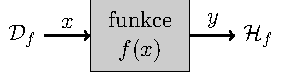
\includegraphics[width=0.45\linewidth]{mai_fig001.pdf}
        \caption{Funkce jako „černá skříňka“. \cite[s.~54]{Musilova2009MA1}}
        \label{mai:fig001}
      \end{figure}
      
      Funkci si podle obrázku \ref{mai:fig001} můžeme představit jako „černou skříňku“, do které 
      vstoupí hodnota (vzor) a vystoupí z ní hodnota \(y = f(x)\) (obraz). Množinu uspořádaných 
      dvojic čísel \([x, f(x)]\) nazveme \textbf{grafem funkce}.
      
      Jak zadat předpis \(f\)? Lze to udělat kterýmkoli z následujících způsobů, podle vhodnosti
      nebo snadnosti. Ukážeme jednotlivé možnosti na jednoduchém příkladu, kdy chceme hodnotám 
      proměnné \(x\) z množiny \(\mathcal{D}_f\) přiřadit jejich druhé mocniny. Zvolme pro náš 
      příklad definiční obor výčtem:
      \begin{equation*}
         \mathcal{D}_f = \lbrace-3,2,-1,0,1,2,3,4\rbrace,
      \end{equation*}
      a zadáme předpis
      \begin{itemize}[noitemsep]
        \item \textbf{slovním popisem}: předpis \(f\) přiřazuje každé z hodnot \(x\in 
              \mathcal{D}_f\) její druhou mocninu,
        \item \textbf{vzorcem}: \(y = x^2\) pro \(x\in \mathcal{D}_f\) zadává zobrazení
              \begin{equation*}
                f: x\in \mathcal{D}_f \rightarrow f(x)= x^2\in\realset,
              \end{equation*}
        \item \textbf{tabulkou}: Hodnoty obrazů pro všechny vzory z \(\mathcal{D}_f\) vypíšeme do 
              tabulky:
              \begin{table}[ht!]
                \centering
                \begin{tabular}{c|rrrrrrrr}
                  \textbf{x} & -3 & -2 & -1 & 0 & 1 & 2 & 3 & 4  \\ \hline
                  \textbf{y} & 9  & 4  & 1  & 0 & 1 & 4 & 9 & 16
                \end{tabular}
                % \caption{ }
              \end{table}
              Proměnná $x$ se v tomto případě mění \uv{diskrétně}. Je zřejmé, že tímto způsobem 
              můžeme funkci definovat úplně jen tehdy, je-li definiční obor konečná množina. 
              Tabulku však používáme i v jiných případech, zejména chceme-li vyznačit pomocí ní, 
              některé hodnoty, které nás z nějakého důvodu přednostně zajímají. 
        \item Zadání \textbf{grafem}: 
          \begin{equation*}
            G_f = \left\lbrace\left[x,f(x)\right] \lvert x\in D\right\rbrace
                = \left\lbrace\left[x,x^2 \right] \lvert x\in D\right\rbrace
          \end{equation*}
          tak, že dvojice \([x, f(x)]\) znázorníme jako body v rovině (obr. \ref{MAI:fig_011}).
          \begin{figure}[ht!]
            \centering  
            \subcaptionbox{\label{MAI:fig_011}}{\luafigure[0.45]{mai_fig002.pdf}}
            \subcaptionbox{\label{MAI:fig_010}}{\luafigure[0.45]{mai_fig003.pdf}}
            \caption{Zadání funkce grafem}
          \end{figure}
          Z grafu můžeme ovšem funkční hodnoty určit pouze přibližně. Pro další matematické 
          zpracování je grafické zadání nejméně vhodné, i když jeho praktický význam například v 
          technických aplikacích nelze popřít.
        \item Zadání pomocí \textbf{rovnice}, jíž je funkce řešením: některé funkce nelze jednoduše 
              zapsat pomocí některého z předchozích způsobů, nebo to alespoň nejde přesně. Lze však 
              zapsat (diferenciální) rovnici, kterou tato funkce splňuje. Jedná se většinou o 
              speciální funkce, jimž se v tomto textu nebudeme věnovat. (Někdy může být taková 
              rovnice  představující zadání funkce i velmi jednoduchá. Například dosti známá funkce 
              \(\erf(x)\), \emph{error funkce}, velmi úzce souvisí s funkcí \(f(x) = 
              \frac{2}{\sqrt{x}}e^{-x^2}\). Nelze ji však zapsat vzorcem. Některé její hodnoty v 
              nejčastěji používaném rozsahu proměnné \(x\) můžeme najít v rozsáhlých tabulkách, 
              které byly sestaveny pomocí numerických metod.)
      \end{itemize}
      
      Již bylo zmíněno, že zadání definičního oboru je neopominutelnou součástí zadání funkce. 
      Kdybychom například zadali funkci opět předpisem \(y=x^2\), avšak za definiční obor stanovili 
      uzavřený interval \(D = \lbrace -3,4\rbrace\), dostali bychom graf na obrázku 
      \ref{MAI:fig_010}. Jde skutečně o jinou funkci než na obrázku \ref{MAI:fig_011}. Její úplnou 
      tabulku bychom nedokázali napsat vůbec.
      
%      Nejčastější způsob zadání funkce představuje \emph{vzorec}. Tabulku alespoň pro některé 
%      hodnoty z \(\mathcal{D}_f\) si pak dokážeme sestavit a schematický graf nakreslit. Někdy se 
%      objeví zadání funkce jen v podobě vzorce, například: „Je dána funkce \(y = f(x)\).“ Znamená 
%      to, že autor zapomněl zadat definiční obor? Nemusí tomu tak být. Tento způsob zadání chápeme 
%      tak, že si sami musíme stanovit „co největší“ definiční obor této funkce, tj. určit množinu 
%      všech takových \(x\), pro která lze do vzorce dosadit a hodnotu \(y\) určit.

      Zobrazovací předpis, kterým je funkce zadána, může být rozmanitý. Nejčastěji a pro účely 
      matematické analýzy nejvhodnější je \emph{analytické zadání vzorcem}, tj. rovnicí tvaru 
      $y=f(x)$ nebo několika takovými rovnicemi platnými pro různé části definičního oboru. Přitom 
      v rovnici $y=f(x)$ je na pravé straně nějaký správně definovaný výraz obsahující nejvýše 
      proměnnou $x$ a nabývající jednoznačné hodnoty pro danou hodnotu proměnné $x$.
      
%      Někdy však používáme (poněkud nedůsledně) termíny \uv{funkce \(f(x)\)} nebo \uv{funkce 
%      \(y=f(x)\)}. V tomto smyslu nepojímáme již \(x\) jako pevný prvek z definičního oboru, ale 
%      jako \uv{nezávisle proměnnou} neboli \emph{argument}, tj. symbol zastupující libovolný prvek 
%      z definičního oboru. V tomto případě pak písmeno \(y\) v rovnici \(y=f(x)\) nazýváme 
%      \emph{závisle proměnnou} a říkáme, že \uv{\(y\) závisí na \(x\)}. Tato frazeologie má své 
%      historické kořeny; tento způsob vyjádření funkce budeme využívat zřídka, zejména tam, kde 
%      nechceme pro označení příslušné funkce zavádět zvláštní symbol. Tak např. budeme mluvit o 
%      funkci \(e^x\) (ačkoliv se zavádí pro exponenciální funkci symbol exp) nebo o funkci \(\sin 
%      x\) (ačkoliv by bylo důslednější mluvit o funkci \(\sin\)) apod. \cite[s.~82]{Brabec1989} 

    %-------------------------------------
      % !TeX spellcheck = cs_CZ
\begin{mdframed}[style=mdexam]
  \begin{example}\label{MAI:exam017}
    (Definiční obor a obor hodnot funkce): Určíme „co největší“ definiční obor funkce
    \(y=\log_2{(\sqrt{1-x^2})}\) a zjistíme také její obor hodnot.
        
    {\centering
    \captionsetup{type=figure}
  %   % !TeX spellcheck = cs_CZ
% exam017.tex
% K příkladu \ref{fyz:fey_exam017} \(y=\log_2{(\sqrt{1-x^2})}\) 

\documentclass[11pt]{standalone}
\usepackage{xltxtra}
\usepackage[usenames,x11names]{xcolor}
\usepackage{tikz}
\usepackage{pgfplots}
  \pgfplotsset{compat=newest}
\usepackage{amsmath}

\begin{document}
  \begin{tikzpicture}[thick,scale=0.7, every node/.style={transform shape}]
    \begin{axis}[
      xmin = -1, xmax = 1, ymin = -10, ymax = 0,
      domain = -0.999999:0.999999,
      restrict y to domain=-30:0,
      grid = major,   % both
      grid style={line width=.1pt, draw=gray!20},
      major grid style={dashed, line width=.2pt, draw=gray!40},
      minor tick num=5,
      clip = true,
      clip mode=individual,
      axis x line = middle,
      axis y line = middle,
      xlabel={\(x\)},
    %  xlabel style={at=(current axis.right of origin), anchor=west},
      ylabel={\(y\)},
    %  ylabel style={at=(current axis.above origin), anchor=south},
      enlarge y limits={rel=0.13},
      enlarge x limits={rel=0.07},
    ]
    
     \addplot[color=Gold3, samples=1000, smooth, ultra thick, unbounded coords=jump, no markers] 
        gnuplot{log10(sqrt(1-x^2))/log10(2)};  
    \end{axis}
  \end{tikzpicture}

\end{document}

% note: předchozí varianta MAI013
%\begin{tikzpicture}
%    \begin{axis}[
%        axis lines=middle,
%        width=10cm, height=10cm,     % size of the image
%        grid = both,
%        grid style={dashed, gray!30},
%        enlargelimits=true,
%        xmin=-1,      % start the diagram at this x-coordinate
%        xmax= 1,      % end   the diagram at this x-coordinate
%        ymin= -6,     % start the diagram at this y-coordinate
%        ymax= 0.5,     % end   the diagram at this y-coordinate
%        /pgfplots/xtick={-1,-0.5,...,1},   % make steps of length 0.2
%        /pgfplots/ytick={0,-0.5,...,-6},   % make steps of length 0.1
%        axis background/.style={fill=white},
%        axis line style={thick, shorten >=2pt, ->, > = {Latex[scale=1.3]}},
% %       every axis x label/.style={
% %        at={(ticklabel* cs:1.0)},
% %        anchor=west,
% %       },
% %       every axis y label/.style={
% %        at={(ticklabel* cs:1.0)},
% %        anchor=south,
% %       },
%        every axis x label/.style={at={(current axis.right of origin)},anchor=west},
%        every axis y label/.style={at={(current axis.north)},above=0mm},
%        ylabel=\(y\),
%        xlabel=\(x\),
% %       title={Dirichletova funkce}
%      ]
%      \addplot[domain=-0.9999:0.9999, line width=0.5pt,samples=1000,red]{log2(sqrt(1-x^2))};
%    \end{axis} 
%\end{tikzpicture}
    \luafigure[0.9]{mai_fig004.pdf}
    \captionof{figure}{K příkladu \ref{MAI:exam017} \(y=\log_2{(\sqrt{1-x^2})}\) 
    \cite[s.~57]{Musilova2009MA1}
    \label{mai:fig004}}
    \par}
    
    Využijeme našich znalostí ze střední školy. Ve hře jsou tři funkce: logaritmus, odmocnina a
    kvadratická funkce, postupně: 
    \begin{equation*}
      y = \log_2w, \qquad w = \sqrt{u}, \qquad u = 1 - x^2.
    \end{equation*}
    „Největším“ definičním oborem logaritmu je množina \(\mathcal{D}(log) = {w\realset \mid w >
    0}\). Oborem hodnot logaritmu pro \(w \in \mathcal{D}(log)\) je celá reálná osa. Hodnoty \(w\)
    však dostáváme vyčíslením odmocniny, která pro přípustné hodnoty \(u\), \(\mathcal{D}(\sqrt{ })
    = \lbrace u\in\realset \lvert u\geq 0\rbrace\), může nabývat všech nezáporných hodnot, tj.
    kladných a hodnoty nula (té nabývá pro \(u = 0\)). Hodnotu \(w = 0\) však nesmíme do logaritmu
    dosadit, takže hodnotu \(u = 0\) musíme ihned vyloučit. Hodnoty proměnné \(x\) musíme omezit
    tak, aby kvadratická funkce \(u = 1 - x^2\) nabývala pouze kladných hodnot. Dostáváme tak
    definiční obor funkce \(y = f(x)\) \(\mathcal{D}=\lbrace x\in\realset \lvert -1<x<1\rbrace\),
    neboli otevřený interval \((-1, 1)\). Pro \(x \in \mathcal{D}\) pak funkce \(u(x)\) nabývá
    hodnot v intervalu \(\mathcal{H}_u = \left( 0, 1\right]\) a funkce \(\log_2\sqrt{1-x^2}\) hodnot
    v intervalu \(\mathcal{H}_u = \left( -\infty, 0\right]\), který je tedy jejím oborem hodnot.
    Graf funkce vidíme na obr. \ref{mai:fig004}. 
  \end{example}
\end{mdframed}
    %-----------------------------------------------------------------------------------------------
    \subsection{Graf funkce}\label{mai:IchapIIIsecIssecII}\hypertarget{mai:IchapIIIsecIssecII}
      Jinými slovy, v předchozím odstavci, bylo řečeno, že každé funkci můžeme přiřadit její graf, 
      a že \textbf{grafem funkce} $f:A\rightarrow\realset,\ A\subset\realset$, rozumíme množinu 
      všech bodů euklidovské roviny, jejíž souřadnice $x$, $y$ v dané kartézské soustavě souřadnic 
      vyhovuje rovnice 
      \begin{equation}\label{mai:eq026}
        y=f(x). 
      \end{equation}  
      
      Graf funkce může v jednodušších případech posloužit jako prostředek k získání názorné 
      \uv{představy}. Grafy některých funkcí jsou \uv{křivky}, (intuitivním smyslu tohoto slova). 
      Avšak u některých funkcí názorná představa grafu selhává. Vezmeme-li např. Dirichletovu 
      funkci, snadno zjistíme, že její graf nemůžeme sestrojit (obr. \ref{mai:fig005} tedy 
      není grafem funkce, ale pouze pokusem o názorné přiblížení Dirichletovi funkce)
      
      \luagraphic[0.8]{mai_fig005.pdf}{Pokus o zobrazení Dirichletovy funkce: \uv{dvě rovnoběžné
      přímky $y=0$ a $y=1$ s nekonečným množstvím mezer}}{mai:fig005}
  
      Z předchozí kapitoly také víme, že zadat funkci znamená udat její definiční obor a 
      \uv{zobrazovací předpis}, tj pravidlo (formulované slovně či v používaném matematickém 
      jazyku), podle něhož můžeme jednoznačným způsobem rozhodnout, jaká funkční hodnota odpovídá 
      libovolně zvolenému číslu z definičního oboru. Definičním oborem bývá často interval nebo 
      sjednocení intervalů. Není-li definiční obor udán, rozumíme jím množinu všech reálných čísel, 
      pro něž je příslušný předpis definován. Tuto množinu nazýváme \textbf{přirozeným} (též 
      maximálním) definičním oborem funkce. Je to tzv. \emph{existenční obor} výrazu, jímž je 
      funkce definována \cite[s.~84]{Brabec1989}.
      
      Například funkce $f: \realset\rightarrow\realset,\ f(x)=x^2$, můžeme vyjádřit bez udání 
      definičního oboru $\realset$ vztahem 
      \begin{equation*}
        f: y=x^2,
      \end{equation*}
      neboť předpis $y=x^2$ má smysl pro každé reálné číslo $x$. Avšak u funkce $g:\langle0, 
      1\rangle\rightarrow\realset,\ g(x)=x^2,$ je nutné v zápisu funkce definiční obor $\langle0, 
      1\rangle$ 
      uvést, píšeme tedy   
      \begin{equation*}
        g: y=x^2, \quad x\in\langle0,1\rangle.
      \end{equation*}
       
      %-------------------------------------
        % !TeX spellcheck = cs_CZ
\wikitextrule
\begin{example}\label{MAI:exam018} 
  Vzorcem $f(x)=\sqrt{1-x}$ je dána funkce, jejímž přirozeným oborem je interval 
  $(-\infty,1\rangle$ (uvažme, že výraz $\sqrt{1-x}$ je definován v reálném oboru, je-li 
  $1-x\geq0$). Graf této funkce je část paraboly, jejíž osou je osa $x$, viz obr. 
  \ref{mai:fig006}.
  
  {\centering
   \captionsetup{type=figure}
%  % !TeX spellcheck = cs_CZ
% mai_fig006.tex

\documentclass[11pt]{standalone}
\usepackage{xltxtra}
\usepackage[usenames,x11names]{xcolor}
\usepackage{tikz}
\usepackage{pgfplots}
  \pgfplotsset{compat=newest}
\usepackage{amsmath}


\begin{document}
  \begin{tikzpicture}[thick,scale=0.7, every node/.style={transform shape}]
    \begin{axis}[
      xmin = -3, xmax = 1.5, ymin = 0, ymax = 3,  % osy
      domain = -3:1,
      restrict y to domain=0:4,
      grid = major,   % both
      grid style={line width=.1pt, draw=gray!20},
      major grid style={dashed, line width=.2pt, draw=gray!40},
      minor tick num=5,
      clip = true,
      clip mode=individual,
      axis x line = middle,
      axis y line = middle,
      xlabel={\(x\)},
    %  xlabel style={at=(current axis.right of origin), anchor=west},
      ylabel={\(y\)},
    %  ylabel style={at=(current axis.above origin), anchor=south},
      enlarge y limits={rel=0.13},
      enlarge x limits={rel=0.07},
    ]
    
     \addplot[color=Gold3, samples=200, smooth, ultra thick, unbounded coords=jump, no markers] 
        gnuplot{sqrt(1-x)};  
    \end{axis}
  \end{tikzpicture}
\end{document} 
   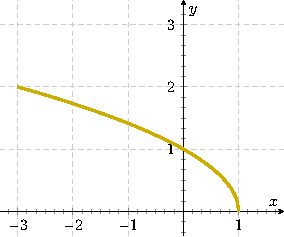
\includegraphics[width=0.5\linewidth]{mai_fig006.pdf}
   \captionof{figure}{{Graf funkce $y=\sqrt{1-x}$ je část paraboly, jejíž hlavní osou je osa $x$}}
   \label{mai:fig006}
   \par}

\end{example}
      %-------------------------------------
      
      %-------------------------------------
        % !TeX spellcheck = cs_CZ
\begin{mdframed}[style=mdexam]
  \begin{example}\label{MAI:exam019} 
    Funkce je dána vzorcem 
    \begin{equation*}
      f(x):y=\abs{x}.
    \end{equation*} 
    Přirozeným definičním oborem této funkce je množina $\realset$. Táž funkce může být dána i 
    vzorcem
    \begin{equation*}
      f(x):y=\sqrt{x^2},
    \end{equation*}    
    nebo dvěma rovnicemi
    \begin{equation*}
      f(x):y=
        \begin{cases}
             x & \text{je-li} x \geq 0. \\
            -x & \text{je-li} x < 0,
        \end{cases}                 
    \end{equation*}  
    což je zřejmé, uvědomíme-li si jak je definována absolutní hodnota. Graf funkce je na obr. 
    \ref{mai:fig007}.
    
    {\centering
    \captionsetup{type=figure}
  %  % !TeX spellcheck = cs_CZ
% mai_fig007.tex

\documentclass[11pt]{standalone}
\usepackage{xltxtra}
\usepackage[usenames,x11names]{xcolor}
\usepackage{tikz}
\usepackage{pgfplots}
  \pgfplotsset{compat=newest}
\usepackage{amsmath}

\begin{document}
  \begin{tikzpicture}[thick,scale=0.7, every node/.style={transform shape}]
    \begin{axis}[
      xmin = -3, xmax = 3, ymin = 0, ymax = 3,  % osy
      domain = -3:3,
      restrict y to domain=0:3,
      grid = major,   % both
      grid style={line width=.1pt, draw=gray!20},
      major grid style={dashed, line width=.2pt, draw=gray!40},
      minor tick num=5,
      clip = true,
      clip mode=individual,
      axis x line = middle,
      axis y line = middle,
      xlabel={\(x\)},
    %  xlabel style={at=(current axis.right of origin), anchor=west},
      ylabel={\(y\)},
    %  ylabel style={at=(current axis.above origin), anchor=south},
      enlarge y limits={rel=0.13},
      enlarge x limits={rel=0.07},
    ]
    
     \addplot[color=Gold3, samples=200, smooth, ultra thick, unbounded coords=jump, no markers] 
        gnuplot{abs(x)};  
    \end{axis}
  \end{tikzpicture} 
\end{document}
    \luafigure[0.9]{mai_fig007.pdf}
    \captionof{figure}{Graf funkce $y=\abs{x}$}
    \label{mai:fig007}
    \par}
  \end{example}
\end{mdframed}
      %-------------------------------------
      
      Funkce může být analyticky zadána i jinak než vzorcem $y=f(x)$. Časté je \textbf{parametrické 
      vyjadřování}, tj. vyjádření dvojicí rovnic 
      \begin{equation}\label{mai:eq027}
        x=\varphi(t),\ y=\psi(t),\ t\in J,
      \end{equation}
      kde $\varphi, \psi$ jsou funkce definované na množině $J$ ($\ J$ bývá obvykle interval). 
      Proměnná $t$ se nazývá \emph{parametr}: má zde pomocný význam. Zajímá nás totiž vztah mezi 
      $x$ a $y$. Rovnice \ref{mai:eq027} definuje relaci 
      $f\subset\realset\times\realset=\realset^2$:
      \begin{equation*}
        f = \{(x,y)\in\realset^2; \exists t\in J \text{ tak, že } x=\varphi(t),\ y=\psi(t)\}.
      \end{equation*}      
      Tato relace může být za \emph{určitých podmínek jednoznačná} tj. je funkcí z $\realset$ do 
      $\realset$. V tomto případě říkáme, že funkce $f$ je \emph{definována parametricky rovnicemi 
      \ref{mai:eq027}}
      
      %-------------------------------------
        % !TeX spellcheck = cs_CZ
\begin{mdframed}[style=mdexam]
  \begin{example}\label{mai:exam020} 
    Rovnice $x=\cos t,\ y=\sin t\quad t\in\langle0,\pi\rangle$, definují parametricky funkci 
    \begin{equation}
      f: y= \sqrt{1-x^2}, \quad x\in\langle-1,1\rangle,
    \end{equation}
    jejíž grafem je polokružnice, ležící v horní polorovině $\{(x,y)\in\realset^2, y\geq0\}$.
    
    {\centering
    \captionsetup{type=figure}
  %   % !TeX spellcheck = cs_CZ
%Graf funkce \(y=\sqrt{1-x^2}\) je polokružnice

\documentclass[11pt]{standalone}
\usepackage{xltxtra}
\usepackage[usenames,x11names]{xcolor}
\usepackage{tikz}
\usepackage{pgfplots}
  \pgfplotsset{compat=newest}
\usepackage{amsmath}

\begin{document}
  \begin{tikzpicture}[thick,scale=0.7, every node/.style={transform shape}]
    \begin{axis}[
      xmin = -1.2, xmax = 1.2, ymin = 0, ymax = 1.3,  % osy
      domain = -1:1,
      restrict y to domain=0:1,
      unit vector ratio=1 1 1,  % axis equal
      grid = major,   % both
      grid style={line width=.1pt, draw=gray!20},
      major grid style={dashed, line width=.2pt, draw=gray!40},
      minor tick num=5,
      clip = true,
      clip mode=individual,
      axis x line = middle,
      axis y line = middle,
      xlabel={\(x\)}, ylabel={\(y\)},
      enlarge y limits={rel=0.07},
      enlarge x limits={rel=0.07},
    ]
    
      \addplot[color=Gold3, samples=200, smooth, ultra thick, unbounded coords=jump, no markers] 
         gnuplot{sqrt(1-x^2)};  
    \end{axis}
  \end{tikzpicture} 
\end{document}
    \luafigure[0.9]{mai_fig008.pdf}
    \captionof{figure}{Graf funkce \(y=\sqrt{1-x^2}\) je polokružnice}
    \label{mai:fig008}
    \par}
  \end{example}
\end{mdframed}
      %-------------------------------------
      
      Blíže se parametrickým zadáním funkce budeme zabývat v kapitole \ref{mai:IchapVI}
      (Aplikace diferenciálního počtu).
      
      Funkce může být někdy zadána též rovnicí tvaru 
      \begin{equation}\label{mai:eq028}
        F(x,y) = 0.
      \end{equation}
      Přitom $F$ je funkce dvou proměnných, tj. zobrazení z $\realset^2\rightarrow\realset$. Kromě 
      rovnice \ref{mai:eq028} může být dána ještě podmínka, aby bod $(x,y)$ patřil k některé 
      množině $M\subset\realset^2$. Rovnicí \ref{mai:eq028} je definována opět jakási relace 
      $f\subset\realset\times\realset$,
      \begin{equation}
        f = \{(x,y)\in\realset^2,\quad F(x,y)=0 \}
      \end{equation}
      (případně $f = \{(x,y)\in\realset^2,\ F(x,y)=0,\ (x,y)\in M \}$), zajímá nás, kdy tato relace 
      je funkcí z $\realset$ do $\realset$. Říkáme pak, že funkce $f$ je dána \textbf{implicitně} 
      uvedenou rovnicí \ref{mai:eq028} (příp. rovnicí \ref{mai:eq028} a podmínkou $(x,y)\in 
      M$). Naproti tomu zadání funkce ve tvaru $y=f(x)$ nazýváme \textbf{explicitním}.

      %-------------------------------------
        % !TeX spellcheck = cs_CZ
\begin{mdframed}[style=mdexam]
  \begin{example}\label{MAI:exam022}\todo[inline]{Nedokončený příklad}
    \begin{itemize}
    \item[]
    \item  Rovnicí $x+2y-3=0$ je implicitně definována funkce  
          $f:y=-\dfrac{1}{2}x+\dfrac{3}{2}$.
    \item  Rovnicí $x^2+y^2=1$ a podmínkou $y\geq0$ je definována implicitní funkce z příkladu 
          \ref{MAI:exam020}. Relace $\{(x,y)\in\realset^2;\ x^2+y^2=1\}$ není ovšem jednoznačná, 
          každé hodnotě $x\in(-1,1)$ odpovídají dvě hodnoty $y: y_1=\sqrt{1-x^2}$, $y: y_2 = 
          -\sqrt{1-x^2}$. Podmínkou $y\geq0$ druhou hodnotu vylučujeme. Místo podmínky $y\geq0$ 
          bychom mohli uvést i jiné podmínky, aby rovnice $x^2+y^2=1$ určovala implicitní funkci.   
    \end{itemize}
  \end{example}
\end{mdframed}
      %-------------------------------------
      
      Vyšetřování podmínek, při nichž rovnice $F(x,y)=0$ je definována funkce $f$, se obvykle 
      provádí metodami matematické analýzy funkce více proměnných. 
          
    %---------------------------------------------------------------------------------------------- 
    \subsection{Vlastnosti funkcí}\label{mai:IchapIIIsecIssecIII}
      \subsubsection{Omezená funkce}
        \begin{definition}\label{MA1:def_lim01}
          Funkci $f$ nazýváme shora (zdola) omezenou na množině $A\subset D(f)$, je-li shora 
          (zdola) omezená množina funkčních hodnot $f(A)$. Je-li funkce $f$ omezená shora i zdola 
          na množině $A$, pak ji nazýváme omezenou na množině $A$. Je-li $A=D(f)$, nazýváme funkci 
          omezenou. Viz kniha \cite[s.~87]{Brabec1989}       
        \end{definition}
        Funkce \(f\) je omezená na množině \(A\), právě když existuje číslo \(K>0\) tak, že platí
        \begin{align*}
         \lvert f(x)\rvert  &\leq K \qquad \text{pro každé } x\in A   \\ 
         \shortintertext{neboli}
         -K\leq f(x) &\leq K \qquad \text{pro každé } x\in A. 
        \end{align*}

        %-------------------------------------
          % !TeX spellcheck = cs_CZ
\wikitextrule
\begin{example}\label{MAI:exam023}
  Funkce $f:y=\dfrac{1}{x^2+1}$ je omezená. Platí totiž 
  \begin{equation*}
    \left|\frac{1}{x^2+1}\right|=\frac{1}{x^2+1}\leq1 \qquad \text{pro všechna }x\in\realset.
  \end{equation*}
  Zdola je tato funkce omezena dokonce číslem $0$.  
\end{example}
        %-------------------------------------

        \begin{itemize}[noitemsep]
          \item Je-li funkce $f$ shora omezená na množině $A$, existuje konečné \emph{supremum}     
                $\sup f(A)$. Toto číslo nazýváme \emph{supremem funkce $f$ na množině $A$} a 
                označujeme je též $\sup_{x\in A}f(A)$ nebo $\sup\{f(x), x\in A\}$.
          \item Je-li funkce $f$ zdola omezená na množině $A$, existuje konečné \emph{infimum} 
                $\inf(A)$, které nazýváme \emph{infimum funkce $f$ na množině $A$} a označujeme je 
                též $\inf_{x\in A}f(A)$ nebo $\inf\{f(x), x\in A\}$. 
          \item Není-li funkce $f$ shora (zdola) omezená na množině $A$, pak je ovšem $\sup_{x\in A}
                f(x)=+\infty$ ($\sup_{x\in A} f(x)=-\infty$).
          \item Má-li množina $f(A)$ největší (nejmenší) prvek, pak toto číslo nazýváme největší 
                (nejmenší hodnotou funkce $f$  na množině $A$ (je-li $A = f(f)$, též absolutním 
                maximem, resp. absolutním minimem funkce $f$) a značíme je $\max_{x\in A} f(x)$ 
                ($\min_{x\in A} f(x)$). V tomto případě existuje takové číslo $x_0\in A$, že 
                $f(x_0)=\max_{x\in A}f(x)$ ($f(x_0)=\min_{x\in A}f(x)$). Pro všechna $x\in A$ tedy 
                platí $f(x)\leq f(x_0)$ ($f(x)\geq f(x_0)$). Je zřejmé, že největší (nejmenší) 
                hodnota funkce $f$ na množině $A$, pokud existuje je současně supremem (infimem) 
                funkce $f$ na $A$.
        \end{itemize}

      %-------------------------------------
        % !TeX spellcheck = cs_CZ
\wikitextrule
\begin{example}\label{MAI:exam021} 
  Pro funkci z příkladu \ref{MAI:exam023} platí:
  \begin{align*}
    \sup_{x\in\realset}&=\frac{1}{x^2+1}=\max_{x\in\realset}=\frac{1}{x^2+1}=1;   \\
    \inf_{x\in\realset}&=\frac{1}{x^2+1}=0,
  \end{align*}
  tato funkce však nenabývá v definičním oboru $\realset$ nejmenší hodnoty, neboť je stále 
  $\dfrac{1}{x^2+1}>0$. To, že infimum je $0$, dokážeme takto: Zvolíme-li libovolně 
  $\varepsilon>0$, pak snadno zjistíme, že existuje $x$, pro něž 
  $\dfrac{1}{x^2+1}<\varepsilon$:
  \begin{align*}
    1                  &< \varepsilon(x^2+1) \\
    \frac{1}{\epsilon} &< x^2+1 \Rightarrow \sqrt{\frac{1}{\epsilon}-1} < x
  \end{align*} 
  
  {\centering
   \captionsetup{type=figure}
%   % !TeX spellcheck = cs_CZ
%Graf funkce $f(x):y=\dfrac{1}{1+x^2}$

\documentclass[11pt]{standalone}
\usepackage{xltxtra}
\usepackage[usenames,x11names]{xcolor}
\usepackage{tikz}
\usepackage{pgfplots}
  \pgfplotsset{compat=newest}
\usepackage{amsmath}

\begin{document}
  \begin{tikzpicture}[thick,scale=0.7, every node/.style={transform shape}]
    \begin{axis}[
      xmin = -4.2, xmax = 4.5, ymin = 0, ymax = 1.3,  % osy
      domain = -4:4,
      restrict y to domain=0:1,
  %    unit vector ratio=1 1 1,  % axis equal
      grid = major,   % both
      grid style={line width=.1pt, draw=gray!20},
      major grid style={dashed, line width=.2pt, draw=gray!40},
      minor tick num=5,
      clip = true,
      clip mode=individual,
  %    /pgfplots/xtick={-2,-1,1,2}, % make steps of length 0.2
      axis x line = middle,
      axis y line = middle,
      xlabel={\(x\)}, ylabel={\(y\)},
      enlarge y limits={rel=0.07},
      enlarge x limits={rel=0.07},
    ]
    
      \addplot[color=Gold3, samples=200, smooth, ultra thick, unbounded coords=jump, no markers] 
         gnuplot{1/sqrt(1+x^2)};  
    \end{axis}
  \end{tikzpicture}
\end{document} 
   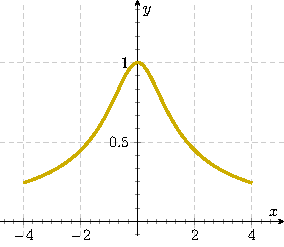
\includegraphics[width=0.5\linewidth]{mai_fig009.pdf}
   \captionof{figure}{Graf funkce $f(x):y=\dfrac{1}{1+x^2}$}
   \label{mai_fig009}
  \par}
  
  Neexistuje tedy kladné číslo, jež by bylo dolní mezí množiny funkčních hodnot, takže infimum je 
  $0$. Graf funkce $f$ je na obr. \ref{mai_fig009}.
\end{example}
      %-------------------------------------
       
      \subsubsection{Monotonní funkce}
        \begin{definition}\label{MA1:def_lim02}
          Funkci $f$ nazýváme \textbf{rostoucí (klesající)} na množině $A\subset D(f)$, jestliže 
          pro každé dva body $x_1, x_2\in A,\ x_1<x_2$, platí $f(x_1)<f(x_2)$ ($f(x_1)>f(x_2)$). 
          Funkci $f$ nazýváme \textbf{neklesající (nerostoucí)} na množině $A\subset D(f)$, 
          jestliže pro každé dvě body $x_1, x_2\in A,x_1<x_2$, platí $f(x_1)\leq f(x_2)$ 
          ($f(x_1)\geq f(x_2)$). Rostoucí a klesající funkce (na množině $A$) se nazývají 
          \textbf{ryze monotónní} (na množině $A$), neklesající a nerostoucí funkce (na množině 
          $A$) se nazývají monotónní (na množině $A$).    
        \end{definition}
            
        Z definice je zřejmé, že každá rostoucí funkce je zároveň neklesající a každá klesající 
        funkce je zároveň nerostoucí. Ryze monotónní funkce tvoří tedy podmnožinu množiny 
        monotónních funkcí. 
           
        \begin{example}
          Funkce $y=2x+1$ je \textbf{rostoucí} na intervalu $(-\infty, \infty)$. Platí totiž:
          $x_1<x_2\Rightarrow 2x_1<2x_2\Rightarrow2x_1+1<2x_2+1$.
        \end{example}
        \begin{example}
          Funkce y=[x] je \textbf{neklesající} na intervalu $(-\infty, \infty)$ (viz příklad **). 
        \end{example}
        \begin{example}
          Heavisideova funkce (viz příklad **) je \textbf{neklesající} na intervalu $(-\infty,
          \infty)$ (viz příklad **). 
        \end{example}       
        \begin{example}
          Funkce $y=\abs{x}$ je \textbf{klesající} na intervalu $(-\infty, 0\rangle$ a rostoucí na
          intervalu $\langle0, \infty)$. 
        \end{example}  
            
        \begin{definition}\label{MA1:def_lim03}
          Funkci $f$ nazýváme \textbf{konstantní} na množině $A$, jestliže pro každé dva body $x_1, 
          x_2\in A$, platí $f(x_1)=f(x_2)$. V tom případě existuje reálné číslo $k$ takové, že pro 
          každé $x\in A$ je $f(x)=k$. Je-li $k=0$, mluvíme o nulové funkci na množině $A$. 
        \end{definition} 
          
        Výrok \uv{funkce $f$ je konstantní na množině $A$} zapisujeme též $f(x)=\text{konst na }A$. 
        Funkci konstantní na $\realset$ budeme stručně nazývat \textbf{konstantní funkcí} nebo 
        krátce \textbf{konstantou}. Z textu bude obvykle patrno, interpretujeme-li symbol $k$ jako 
        reálné číslo nebo jako konstantní funkci. Je zřejmé, že konstantní funkce na množině $A$ je 
        zároveň neklesající i nerostoucí na množině $A$. Toto tvrzení se dá obrátit. Lze snadno 
        dokázat i tuto větu:        
        \begin{lemma}\label{MA1:lem_lim01}
          Funkce $f$ je \textbf{rostoucí} na množině $A$, právě když je neklesající na množině $A$ a na žádné dvoubodové podmnožině $B\subset A$ není konstantní. 
        \end{lemma}
        Obdobná tvrzení platí i pro klesající funkce. 
               
      \subsubsection{Sudé a liché funkce}
        \begin{definition}\label{MA1:def_lim04}
          Funkce $f$ se nazývá \textbf{sudá} jestliže pro každé $x\in D(f)$ je též $-x\in D(f)$  a 
          platí $f(x)=f(-x)$.
          Funkce $f$ se nazývá \textbf{lichá} jestliže pro každé $x\in D(f)$ je též $-x\in D(f)$  a 
          platí $f(-x)=-f(x)$. 
        \end{definition}
        Graf sudé funkce je souměrný podle osy $y$ (osy funkčních hodnot), graf liché funkce je  
        souměrný podle počátku. 
 
       %-------------------------------------
         % !TeX spellcheck = cs_CZ
\wikitextrule
\begin{example}\label{MAI:exam024} 
  Funkce $f:\,y=x^2$ je sudá, funkce $g:\,y=x^3$ je lichá.
  
  {\centering
   \begin{tabular}{cc}
     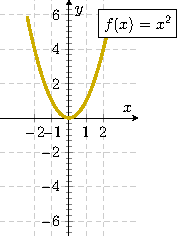
\includegraphics[width=0.5\linewidth]{mai_fig010.pdf}              &
     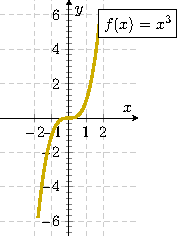
\includegraphics[width=0.5\linewidth]{mai_fig011.pdf}             \\
  \end{tabular}
  \captionsetup{type=figure}
  \captionof{figure}{Příklad sudé a liché funkce}\label{MAI:fig_002}
  \par}
\end{example}
       %-------------------------------------

        Daná funkce nemusí být ovšem ani sudá, ani lichá. Snadno se dokáže tvrzení:
        \begin{itemize}[noitemsep]
          \item Je-li sudá funkce $f$ na množině $D(f)\cap\langle0,\infty)$ rostoucí (klesající),
                je na množině $D(f)\cap(-\infty,0\rangle$ klesající (rostoucí).
          \item Je-li lichá funkce na množině $D(f)\cap\langle0,\infty)$ rostoucí (klesající),
                je též na množině $D(f)\cap(-\infty,0\rangle$ klesající (rostoucí).                 
        \end{itemize}
      \subsubsection{Periodická funkce}

    \subsection{Operace s funkcemi. Uspořádání}\label{mai:IchapIIIsecIssecIV}
      Jak s funkcemi počítat? Definujeme základní operace s nimi - \emph{součet funkcí, součin 
      funkcí a násobení funkce reálným číslem}. Předpokládejme, že na definičním oboru 
      \(\mathcal{D}\) jsou zadány funkce \(f\) a \(g\) a reálné číslo \(\alpha\). Pak na tomtéž 
      definičním oboru lze zadat nové funkce
      \begin{align*}
        \mathcal{F} &: \mathcal{D}\ni x\,\rightarrow\,\mathcal{F}(x) = f(x)+g(x)  \in\realset   \\
        \mathcal{G} &: \mathcal{D}\ni x\,\rightarrow\,\mathcal{G}(x) = \alpha g(x)\in\realset   \\
        \mathcal{H} &: \mathcal{D}\ni x\,\rightarrow\,\mathcal{H}(x) = f(x) g(x)  \in\realset 
      \end{align*}
      Funkce \(\mathcal{F}\), \(\mathcal{G}\) a \(\mathcal{H}\) nazýváme postupně součtem funkcí 
      \(f\) a \(g\), \(\alpha\)-násobkem funkce \(f\) a součinem funkcí \(f\) a \(g\). Značíme
      \begin{equation*}
       \mathcal{F} = f + g, \qquad \mathcal{G} = \alpha f, \qquad \mathcal{H} = fg. 
      \end{equation*}
      
      Všimněme si nyní pravidel pro počítání s funkcemi zadanými na \(\mathcal{D}\) a zjistíme, 
      že se velmi podobají pravidlům pro počítání s reálnými čísly. Není divu, vždyť operace s 
      funkcemi jsou definovány prostřednictvím funkčních hodnot, a těmi jsou reálná čísla. Některé 
      důležité odlišnosti však přece jen najdeme. Napřed ale pravidla:
      
      \begin{itemize}[noitemsep]
        \item komutativní zákon pro součet funkcí
          \begin{equation}\label{mai:eq012}
            f(x) + g(x) = g(x) + f(x)
          \end{equation}
        \item asociativní zákon pro součet funkcí  
          \begin{equation}\label{mai:eq013}
            (f(x) + g(x)) + h(x) = f(x) + (g(x) + h(x)
          \end{equation}
        \item existence univerzálního neutrálního  prvku \(O\) (nulová funkce \(O:\mathcal{D}\ni x 
          \rightarrow O(x)=0\))
          \begin{equation}\label{mai:eq014}
            f(x) + O = O + f(x) = f(x)
          \end{equation}
        \item existence právě jednoho opačného prvku k funkci \(f\), přičemž \((-f)(x) = -f(x)\)
          \begin{equation}\label{mai:eq015}
            f(x)+(-f(x))=(-f(x))+f(x)=O
          \end{equation}
        \item asociativní zákon pro násobení číslem 
         \begin{equation}\label{mai:eq016}
            (\alpha_1\alpha_2)f(x) = \alpha_1(\alpha_2f(x))
         \end{equation}
        \item  1. distributivní zákon pro násobení číslem
          \begin{equation}\label{mai:eq017}
            \alpha(f(x)+g(x) =\alpha f(x) + \alpha g(x)
          \end{equation}\label{mai:eq018}
        \item 2. distributivní zákon pro násobení číslem 
          \begin{equation}\label{mai:eq019}
            (\alpha_1+\alpha_2)f(x) =\alpha_1f(x)+\alpha_2f(x)
          \end{equation}
        \item násobení číslem \((-1)\) dává opačný prvek
          \begin{equation}\label{mai:eq020}
            (-1)f(x)=(-f(x))
          \end{equation}
        \item komutativní zákon pro součin funkcí
          \begin{equation}\label{mai:eq021}
            f(x)g(x)=g(x)f(x)
          \end{equation}
        \item asociativní zákon pro součin funkcí 
          \begin{equation}\label{mai:eq022}
            f(x)(g(x)h(x))=(f(x)g(x))h(x)
          \end{equation}
        \item distributivní zákon zprava pro součin funkcí
          \begin{equation}\label{mai:eq023}
            (f_1(x) + f_2(x))g(x) =f_1(x)g(x) + f_2(x)g(x)
          \end{equation}
        \item distributivní zákon zleva pro součin funkcí
          \begin{equation}\label{mai:eq024}
            f(x)(g_1(x) + g_2(x))=f(x)g_1(x)+f(x)g_2(x)
          \end{equation}
        \item násobení jednotkovou funkcí \(I: \mathcal{D}\ni x \rightarrow I(x) = 1\)  
          \begin{equation}\label{mai:eq025}
           f(x)I=If(x)
          \end{equation}
        \item existence právě jedné \emph{převrácené} funkce k funkci \(f\) pro \(f(x)\neq0\quad 
              (f)^{-1}: \bar{D}\ni x\rightarrow (f)^{-1}(x)=[f(x)]^{-1}\) kde \(\bar{\mathcal{D}} 
              = \mathcal{D} - \left\{x\in \mathcal{D}\,\lvert\,f(x)=0\right\}\)
          \begin{equation}
            f(x)(f(x))^{-1}=(f(x))^{-1}f(x) = I
          \end{equation}
      \end{itemize}
      Všimněme si, že funkce \((f)^{-1}\) existuje obecně na užším definičním oboru 
      \(\bar{\mathcal{D}}\), než na kterém je definována funkce \(f\). Je totiž třeba vyloučit 
      všechny hodnoty \(x\), pro které \(f(x) = 0\) (zákaz dělení nulou). K funkci \(O\) tedy 
      převrácená funkce neexistuje vůbec!
      
      Existence opačné a převrácené funkce k \(f\) umožňuje definovat \emph{rozdíl} a \emph{podíl} 
      funkcí \(f-g=f+(-g)\) a \(\dfrac{f}{g}=f(g)^{-1}\), tj.
      \begin{alignat*}{2}
        f-g         &: \mathcal{D}\ni x\,\rightarrow\, (f-g)(x)&&=f(x)+(-g)(x) \\
                    &                                          &&=f(x)-g(x),  \\
        \frac{f}{g} &: \bar{D}\ni x\,\rightarrow\, 
                                   \left(\frac{f}{g}\right)(x) &&= f(g)^{-1}(x) = \frac{f(x)}{g(x)}, 
      \end{alignat*}
      kde \(\bar{D}=D-\left\{x\in D\,\lvert\,g(x)=0 \right\}\) 
      
      \begin{mdframed}[style=mdnote]
        \begin{note}
          Pamatujme si označení převrácené funkce jako \((f)^{-1}\), v němž je zápis symbolu \(f\)
          do závorky podstatný. Jde o něco jiného než znamená symbol \(f^{-1}\) bez závorky, který
          rezervujeme pro inverzní funkci v dalším výkladu.
        \end{note}
      \end{mdframed}  

      \begin{mdframed}[style=mdnote]
        \begin{note}
          Porovnáme-li nyní vlastnosti operací s funkcemi a pravidla pro počítání s reálným čísly, 
          komplexními čísly, maticemi a vektory, můžeme konstatovat, že množina funkcí s operací 
          sčítání funkcí a násobení funkce číslem je \textbf{vektorovým prostorem}. To je vlastnost, 
          která je s případem čísel, matic a vektorů společná. Vektorový prostor funkcí se však od 
          zmiňovaných vektorových prostorů výrazně liší svou dimenzí (rozměrem). Intuitivně dobře 
          chápeme, co znamená jednorozměrný, dvojrozměrný a trojrozměrný prostor (například 
          \(\realset^1\), \(\realset^2\), \(\realset^3\)). V odstav 1.4 jsme dokonce pracovali v 
          n-rozměrném vektorovém prostoru. Dimenze vektorového prostoru může být i nekonečná - třeba 
          zrovna u funkcí. Obecně jde o pojem poměrně obtížný a budeme se jím důkladně zabývat až v 
          kapitolách věnovaných algebře \cite[s.~58]{Musilova2009MA1}.
        \end{note}
      \end{mdframed}  
      
      Operace s funkcemi jsme definovali a prodiskutovali pro případ, kdy definiční obory funkcí, 
      vstupujících do operace byly stejné. Co když tomu tak nebude? Znamená to, že pak nemůžeme 
      funkce sčítat, násobit, apod.? Předpokládejme, že definičním oborem funkce \(f\) je množina 
      \(\mathcal{D}_f\) definičním oborem funkce \(g\) množina \(D_g\). Pokud jsou tyto obory 
      disjunktní, tj. \(\mathcal{D}_f \cap \mathcal{D}_g = 0\), můžeme utvořit pouze 
      \(\alpha\)-násobek funkce \(f\) či \(g\). Sčítat ani násobit funkce \(f\) a \(g\) nemůžeme 
      neboť hodnota \(f(x) + g(x)\) ani \(f(x)g(x)\) neexistuje pro žádné \(x\). Pokud je průnik 
      \(D=d_f\cap D_g\) oborů \(\mathcal{D}_f\) a \(\mathcal{D}_g\) neprázdný, stává se definičním 
      oborem funkcí \(f+g\) a \(fg\). Platí stejná pravidla jako v předchozí tabulce, pouze s 
      omezením na obor \(\mathcal{D}_f\).
    
    \subsection{Skládání a inverze funkcí}\label{mai:IchapIIIsecIssecV}
      \emph{Skládání} neboli kompozici funkcí si lze snadno představit opět pomocí „černých skříněk
      “ (obr. \ref{mai:fig012}): Do první skřínky představující předpis \(g\), \emph{vnitřní složku}
      složené funkce, vstupuje hodnota \(x\) z definičního oboru \(\mathcal{D}_g\) funkce \(g\).

      \luagraphic[0.9]{mai_fig012.pdf}{Skládání funkcí \cite[s.~59]{Musilova2009MA1}}{mai:fig012}

      Výstupem je číslo \(u = g(x)\), funkční hodnota vnitřní složky v bodě \(x\). Toto číslo smí
      vstoupit do skříňky představující předpis \(f\), \emph{vnější složku} složené funkce, právě
      tehdy, je-li prvkem jejího definičního oboru \(\mathcal{D}_f\). V takovém případě najdeme na
      výstupu ze skříňky \(f\) hodnotu \(y = f(u) = f[g(x)]\). (Jestliže
      \(g(x)\notin\mathcal{D}_f\), není výstup ze skříňky \(f\) definován.) Vzniká nový předpis
      \(F\), kterým se některým bodům definičního oboru \(\mathcal{D}_g\), ne všem, ale pouze těm,
      pro něž \(g(x)\in\mathcal{D}_f\), přiřazují hodnoty \(f[g(x)]\). Definujme nyní složenou
      funkci přesněji: Předpokládejme, že jsou zadány funkce
      \begin{align*}
        g  &: \mathcal{D}_g\ni x\,\rightarrow\, g(x) = u\in\realset, \\
        f  &: \mathcal{D}_f\ni u\,\rightarrow\, f(u) = y\in\realset. \\
        \shortintertext{označme}
        \mathcal{D} &= \{x\lvert x\in\mathcal{D}_g \text{ a současně } g(x)\in\mathcal{D}_f\}.
      \end{align*}
      Pokud \(\mathcal{D} = \emptyset\), lze definovat funkci
      \begin{equation*}
        F: \mathcal{D}\ni x\rightarrow y = F(x) = f[g(x)]\in\realset, 
           \text{ značíme } F = f \circ g.
      \end{equation*}
      \(F\) se nazývá \emph{složením} neboli \emph{kompozicí} funkcí \(g\) a \(f\). Zápis \(f\circ 
      g\) čteme často také jako \emph{„f po g“}. Skládat lze i větší počet funkcí.

       %-------------------------------------
         % !TeX spellcheck = cs_CZ
\begin{mdframed}[style=mdexam]
  \begin{example}\label{MAI:exam025}
    Uvažme funkci z příkladu \ref{vol02:fyz:fey_exam017}. 
    
    {\centering
    \captionsetup{type=figure}
  %   % !TeX spellcheck = cs_CZ
\documentclass[11pt]{standalone}
\usepackage{xltxtra}
\usepackage[usenames,x11names]{xcolor}
\usepackage{tikz}
\usepackage{pgfplots}
  \pgfplotsset{compat=newest}
\usepackage{amsmath}

\begin{document}
  \begin{tikzpicture}[thick,scale=0.7, every node/.style={transform shape}]
    \begin{axis}[
      xmin = -5, xmax = 5, ymin = -10, ymax = 1.5,
   %   domain = -0.999999:0.999999,
      restrict y to domain=-30:1.5,
      unit vector ratio=1 1 1,  % axis equal
      grid = both,   % both, major
      grid style={line width=.1pt, draw=gray!20},
      major grid style={dashed, line width=.2pt, draw=gray!40},
      minor tick num=4,
      clip = true,
      clip mode=individual,
      axis x line = middle,
      axis y line = middle,
      xlabel={$x$},
    %  xlabel style={at=(current axis.right of origin), anchor=west},
      ylabel={$u,w,y$},
    %  ylabel style={at=(current axis.above origin), anchor=south},
      enlarge y limits={rel=0.13},
      enlarge x limits={rel=0.07},
    ]
    
      \addplot[color=Gold3, samples=1000, smooth, ultra thick, unbounded coords=jump, no markers, 
               domain = -0.999999:0.999999] 
        gnuplot{log10(sqrt(1-x^2))/log10(2)};  
        
     \addplot[color=green, samples=200, smooth, ultra thick, unbounded coords=jump, no markers, 
     domain = -3.3:3.3] 
        gnuplot{1-x^2};
        
     \addplot[color=blue, samples=200, smooth, ultra thick, unbounded coords=jump, no markers, 
     domain = -1:1] 
        gnuplot{sqrt(1-x^2)};  
    \end{axis}
  \end{tikzpicture}
\end{document}
    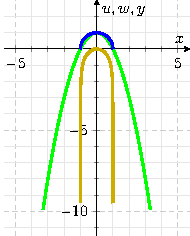
\includegraphics[width=0.6\linewidth]{mai_fig013.pdf}
    \captionof{figure}{K příkladu \ref{MAI:exam025} \(y=\log_2{(\sqrt{1-x^2})}\) 
    \cite[s.~57]{Musilova2009MA1}
    \label{mai:fig013}}
    \par}
    
    Ukážeme, jak tato funkce vzniká postupně složením tří funkcí a jak při tom dochází k postupnému 
    omezování definičního oboru. Písmeny \(\mathcal{D}\) a \(H\) s příslušným indexem budeme značit 
    definiční obory a obory hodnot jednotlivých funkcí.
    \begin{gather*}
      \begin{align*}
        g&:  \realset =\mathcal{D}_g\ni x\rightarrow u=g(x) = 1- x^2  \in\mathcal{H}_g=(-\infty,1], \\
        h&: [0,\infty)=\mathcal{D}_h\ni u\rightarrow w=h(u) = \sqrt{u}\in\mathcal{H}_h=[0,\infty),  \\
       \shortintertext{\(\mathcal{D}_h\cap\mathcal{H}_g = [0,1]\Rightarrow\mathcal{D}_{h\circ g}=[-1,1], 
                       \mathcal{H}_{h\circ g} = [0,1],\)}                                    \\
       f&:(0,\infty)=\mathcal{D}_f\ni w \rightarrow y=f(w)=\log_2w\in\mathcal{H}_f=\realset  \\
       \shortintertext{\(\mathcal{H}_{h\circ g}\cap\mathcal{D}_f = (0,1] 
                       \Rightarrow\mathcal{D}_F=(-1,1),\mathcal{H}_F=(-\infty,0].\)} 
      \end{align*}
    \end{gather*}
    Je tedy
    \begin{gather*}
      \begin{align*}
        F:\mathcal{D}_F\ni x\rightarrow 
        y&=F(x)=(f\circ(h\circ g))(x) = f{h[g(x)]}          \\
        &= \log_2\sqrt{1-x^2}\in(-\infty,0].
      \end{align*}
    \end{gather*}
    Názorněji než tento zápis ukazuje situaci obrázek \ref{mai:fig013}.
  \end{example}
\end{mdframed}
       %-------------------------------------
      
      Může vzniknout otázka, jak rozpoznáme vnitřní a vnější složku složené funkce. Rozlišit 
      vnitřní a vnější složku třeba u funkcí \(\cos(x^2)\) a \((cos x)^2\) není problém. Hned také 
      vidíme, že obecně \(f\circ g\neq g\circ f\), i když by definiční obory funkcí na pravé i levé 
      straně měly neprázdný průnik. Jsou však i případy na první pohled méně zřetelné, jak ukazuje 
      následující příklad.
      
      %-------------------------------------
        % !TeX spellcheck = cs_CZ
\begin{mdframed}[style=mdexam]
  \begin{example}\label{mai:exam026}
    (Určení vnitřní a vnější složky) Uveďme příklad dvou funkcí \(F(x)=\sqrt{x^2}\) a \(G(x) =
    (\sqrt{x})^2\). Liší se tyto funkce, nebo jde o tutéž funkci, jen jinak zapsanou? Vidíme, že
    platí

    \begin{align*}
      \mathcal{D}_F &=\realset, F(x)=\abs{x}\forall x\in\mathcal{D}_F, \mathcal{H}_F = [0, infty),\\
      \mathcal{D}_G &=[0, \infty), G(x)=x\forall    x\in\mathcal{D}_G, \mathcal{H}_G = [0, infty).
    \end{align*}
    Funkce \(F\) a \(G\) mají různé definiční obory, ale na jejich průniku dávají stejné funkční
    hodnoty. Ani zde však obecně nelze pořadí skládání funkcí zaměňovat.
  \end{example}
\end{mdframed}
      %-------------------------------------
       
      Funkce \(F\) a \(G\) mají různé definiční obory, ale na jejich průniku dávají stejné funkční 
      hodnoty. Ani zde však obecně nelze pořadí skládání funkcí zaměňovat.
      
      Nyní se pusťme do vybudování pojmu inverzní funkce k funkci \(f\). Představme si, že funkční
      hodnota \(y = f(x)\) zadané funkce
      \begin{equation*}
        f: \mathcal{D}_f\ni x \rightarrow f(x)\in\mathcal{H}_f
      \end{equation*}
      představuje „zakódovanou“ informaci o hodnotě \(x\). Položme si otázku, zda a za jakých 
      podmínek dokážeme sestavit „černou skříňku“, na jejímž výstupu by se při vstupu obrazu \(y = 
      f(x)\) objevila hodnota \(x\). Omezení takové možnosti je názorně vidět na obrázku 
      \ref{mai:fig014}. V případě funkce \(f(x)\) lze ke všem obrazům \(y \in \mathcal{H}_f\) najít 
      vzory, v případě funkce \(g(x)\) to možné není, neboť jeden a týž obraz lze získat z několika 
      vzorů. Pro který bychom se tedy měli rozhodnout?
      
      \luagraphic[0.9]{mai_fig014.pdf}{Skládání funkcí \cite[s.~61]{Musilova2009MA1}}{mai:fig014}

       Aby bylo možné vzor zpětně identifikovat na základě znalosti obrazu, je třeba, aby funkce 
       \(f\) byla \emph{prostá}, tj. aby předpis \(f\) přiřazoval každým dvěma různým vzorům \(X_1 
       \neq x_2\) dva různé obrazy \(f(x_1) \neq f(x_2)\). Často lze tohoto požadavku docílit tím, 
       že se místo funkce \(f\) s definičním oborem \(\mathcal{D}_f\) spokojíme s funkcí, která 
       vznikne omezením \emph{(restrikcí)} té původní na „menší“ definiční obor, zato však již bude 
       prostá. U funkce \(g\) na obrázku \ref{mai:fig016} by tak stačilo omezit definiční obor 
       například na množinu \(\mathcal{D}_g\). Než inverzní funkci definujeme, ukažme si způsob 
       jejího nalezení na známém příkladu.

       \begin{figure}[ht!]
          \centering  
          \subcaptionbox{\label{mai:fig016a}}{\luafigure[0.45]{mai_fig016a.pdf}}
          \subcaptionbox{\label{mai:fig016b}}{\luafigure[0.45]{mai_fig016b.pdf}}
          \caption{K pojmu inverzní funkce}
          \label{mai:fig016}
       \end{figure}
      
      %-------------------------------------
        % !TeX spellcheck = cs_CZ
\begin{mdframed}[style=mdexam]
  \begin{example}\label{MAI:exam027}
    (Nalezení inverzní funkce): Funkci 
    \begin{equation*}
      y = \log_2(\sqrt{1-x^2})
    \end{equation*}
    Jsme již z různých hledisek rozebrali v příkladech \ref{vol02:fyz:fey_exam017} a
    \ref{MAI:exam025}. Hodí se i nyní.

    {\centering
    \captionsetup{type=figure}
  %  % !TeX spellcheck = cs_CZ
% K příkladu \ref{mai:exam027} \(y=\log_2{(\sqrt{1-x^2})}

\documentclass[11pt]{standalone}
\usepackage{xltxtra}
\usepackage[usenames,x11names]{xcolor}
\usepackage{tikz}
\usepackage{pgfplots}
  \pgfplotsset{compat=newest}
\usepackage{amsmath}

\begin{document}
  \begin{tikzpicture}[thick,scale=0.7, every node/.style={transform shape}]
    \begin{axis}[
      xmin = -5, xmax = 5, ymin = -5, ymax = 1.5,
   %   domain = -0.999999:0.999999,
      restrict y to domain=-30:1.5,
      unit vector ratio=1 1 1,  % axis equal
      grid = both,   % both, major
      grid style={line width=.1pt, draw=gray!20},
      major grid style={dashed, line width=.2pt, draw=gray!40},
      minor tick num=4,
      clip = true,
      clip mode=individual,
      axis x line = middle,
      axis y line = middle,
      xlabel={\(x\)},
    %  xlabel style={at=(current axis.right of origin), anchor=west},
      ylabel={\(y\)},
    %  ylabel style={at=(current axis.above origin), anchor=south},
      enlarge y limits={rel=0.13},
      enlarge x limits={rel=0.07},
    ]
    
      \addplot[color=Gold3, samples=1000, smooth, ultra thick, unbounded coords=jump, no markers, 
               domain = 0:0.9995] 
        gnuplot{log10(sqrt(1-x^2))/log10(2)};  
        
      \addplot[color=blue, samples=200, smooth, ultra thick, unbounded coords=jump, no markers, 
               domain = -5:0] 
        gnuplot{sqrt(1-2^(2*x))};  
    \end{axis}
  \end{tikzpicture}
\end{document}
    \luafigure[0.9]{mai_fig015.pdf}
    \captionof{figure}{K příkladu \ref{MAI:exam027} \(y=\log_2{(\sqrt{1-x^2})}\) 
    \cite[s.~62]{Musilova2009MA1}
    \label{mai:fig015}}
    \par}
    
    Na obrázku \ref{mai:fig013} máme dokonce její graf, a tak vidíme, že \textbf{není} na svém 
    definičním oboru \((-1, 1)\) \textbf{prostá}. Omezme proto její definiční obor na interval 
    \(\mathcal{D} = [0, 1)\), na němž již prostá je (část grafu vpravo od osy \(y\)). Pro danou 
    hodnotu obrazu \(y \in (-\infty,0]\) můžeme již jednoznačně určit hodnotu \(x\) jednoduchou 
    úpravou:
    \begin{align*}
      y = \log_2(\sqrt{1-x^2}) &\Rightarrow \sqrt{1-x^2} = 2^y   \\
                               &\Rightarrow x^2 = 1 - 2^{2y}     \\
                               &\Rightarrow x = \sqrt{1 - 2^{2y}}
    \end{align*}
    Formální záměnou \(x \leftrightarrow y\) dostáváme inverzní funkci k funkci \(f\),
    \begin{equation*}
      y =f^{-1}(x) = \sqrt{1 - 2^{2x}}.
    \end{equation*}
    Grafy obou funkcí jsou na obrázku \ref{mai:fig015}.
  \end{example}
\end{mdframed}
      %-------------------------------------
      
      Ze způsobu konstrukce funkce \(f^{-1}\) v předchozím příkladu je vidět, že 
      \(\mathcal{D}_{f^{-1}} = \mathcal{H}_f\), \(\mathcal{H}_{f^{-1}} = \mathcal{D}_f\) a graf 
      inverzní funkce je obrazem grafu prosté funkce \(f\) při osové symetrii v rovině 
      souřadnicových os vzhledem k ose prvního a třetího kvadrantu. Nyní již definujeme inverzní 
      funkci obecně. Předpokládejme, že funkce \(f : \mathcal{D}_f\ni x \rightarrow y = f(x)\ni 
      \mathcal{H}_f\) je prostá na svém definičním oboru. Pak existuje funkce \(f^{-1}\) definovaná 
      jako
      \begin{equation}\label{mai:eq029}
        f^{-1} :\mathcal{H}_f\ni x\rightarrow y = f^{-1}(x)\in\mathcal{D}_f\Leftrightarrow x = f(y).
      \end{equation}
      Funkci \(f^{-1}\) nazýváme \textbf{inverzní funkcí k funkci} \(f\). Ještě shrneme pravidla 
      pro skládání funkcí a pro inverzní funkce:

      \begin{itemize}[noitemsep]
        \item asociativní zákon pro skládání funkcí
          \begin{equation}\label{mai:eq030}
            f(x)\circ(h(x)\circ g(x)) = f(x)\circ h(x) \circ g(x)
          \end{equation}
        \item distributivní zákon zleva 
          \begin{equation}\label{mai:eq031}
            f(x) \circ (h(x) + g(x)) = f(x) \circ h(x) + f(x) \circ g(x)
          \end{equation}
        \item existence univerzálního neutrálního  prvku \(O\) (nulová funkce \(O:\mathcal{D}\ni x 
          \rightarrow O(x)=0\))
          \begin{equation}\label{mai:eq032}
            f(x) + O = O + f(x) = f(x)
          \end{equation}
        \item existence právě jednoho opačného prvku k funkci \(f\), přičemž \((-f)(x) = -f(x)\)
          \begin{equation}\label{mai:eq033}
            f(x)+(-f(x))=(-f(x))+f(x)=O
          \end{equation}
        \item komutativní zákon pro součet funkcí
          \begin{equation}\label{mai:eq034}
            f(x) + g(x) = g(x) + f(x)
          \end{equation}
        \item asociativní zákon pro součet funkcí  
          \begin{equation}\label{mai:eq035}
            (f(x) + g(x)+h(x) = f(x) + (g(x) + h(x)
          \end{equation}
        \item existence univerzálního neutrálního  prvku \(O\) (nulová funkce \(O:\mathcal{D}\ni x 
          \rightarrow O(x)=0\))
          \begin{equation}\label{mai:eq036}
            f(x) + O = O + f(x) = f(x)
          \end{equation}        
      \end{itemize}   
      Předchozí vztahy platí na patřičně zúžených definičních oborech funkcí, které do nich 
      vstupují.
      
  %-------------------------------------------------------------------------------------------------
  \section{Zvěřinec funkcí}\label{mai:IchapIIIsecII}
    Základními elementárními funkcemi nazýváme \cite[s.~10]{PolakMA1}:
    %------------- Goniometrické funkce ------------------------------------------------------------
    \subsection{Goniometrické funkce}  
    \begin{itemize}
      \item \textbf{Základní vzorce pro goniometrické funkce}
        \begin{align}
          \sin^2\alpha     &+ \cos^2\alpha = 1      &\forall\alpha\in\realset \label{MA1:eq_sincos} \\ 
          \abs{\sin\alpha} &= \sqrt{1-\cos^2\alpha} &\forall\alpha\in\realset \label{MA1:eq_sinabs} \\ 
          \abs{\cos\alpha} &= \sqrt{1-\sin^2\alpha} &\forall\alpha\in\realset \label{MA1:eq_cosabs}
        \end{align}  
      \item \textbf{Součtové vzorce}
        \begin{align}
        % \nonumber to remove numbering (before each equation)
          \sin(\alpha + \beta) 
            &= \sin\alpha\cdot\cos\beta 
             - \sin\beta\cdot\cos\alpha           \label{MA1:eq_sinxpy}  \\ 
          \sin(\alpha - \beta) 
            &= \sin\alpha\cdot\cos\beta 
             + \sin\beta\cdot\cos\alpha           \label{MA1:eq_sinxmy}  \\ 
          \cos(\alpha + \beta) 
            &= \cos\alpha\cdot\cos\beta 
             - \sin\alpha\cdot\sin\beta           \label{MA1:eq_cosxpy}  \\ 
          \cos(\alpha - \beta) 
            &= \cos\alpha\cdot\cos\beta 
             + \sin\alpha\cdot\sin\beta           \label{MA1:eq_cosxmy}  \\ 
          \tan(\alpha\pm\beta) 
            &= \frac{\tan\alpha\pm\tan\beta}{1\mp\tan\alpha\cdot\tan\beta} \label{MA1:eq_tanxpmy}\\ 
          \cot(\alpha\pm\beta) 
            &= \frac{1\mp\cot\alpha\cdot\cot\beta}{\cot\alpha\pm \cot\beta} \label{MA1:eq_cotxpmy}
        \end{align}
        Součtové vzorce lze odvodit několika způsoby; jednoduchý způsob důkazu
        lze provést pomocí skalárního součinu vektorů.
      \item \textbf{Vzorce pro dvojnásobný úhel $2\alpha$}
        \newline Pro každé $\alpha\in R$ platí:
        \begin{align}
          \sin(2\alpha)   &= 2\sin\alpha\cos\alpha                \label{MA1:eq_sin2x} \\ 
          \cos(2\alpha)   &= \cos^2\alpha - \sin^2\alpha          \label{MA1:eq_cos2x} \\ 
          \tan(2\alpha)   &= \frac{2\tan\alpha}{1-\tan^2\alpha}   \label{MA1:eq_tan2x} \\ 
          \cot(2\alpha)   &= \frac{\cot^2\alpha - 1}{2\cot\alpha} \label{MA1:eq_cot2x}
        \end{align}
      \item \textbf{Vzorce pro poloviční úhel $\displaystyle\frac{\alpha}{2}$}
        \begin{align}
          \left\lvert\sin\frac{\alpha}{2}\right\rvert   
            &= \sqrt{\frac{1-\cos\alpha}{2}}                      \label{MA1:eq_sinx2} \\ 
          \left\lvert\cos\frac{\alpha}{2}\right\rvert   
            &= \sqrt{\frac{1+\cos\alpha}{2}}                      \label{MA1:eq_cosx2} \\ 
          \left\lvert\tan\frac{\alpha}{2}\right\rvert   
            &= \sqrt{\frac{1-\cos\alpha}{1+\cos\alpha}}           \label{MA1:eq_tanx2} \\ 
          \left\lvert\cot\frac{\alpha}{2}\right\rvert   
            &= \sqrt{\frac{1+\cos\alpha}{1-\cos\alpha}}           \label{MA1:eq_cotx2}
        \end{align}
    \end{itemize}
    Vzorce \ref{MA1:eq_sinx2} a \ref{MA1:eq_cosx2} odvodíme pomocí vzorců \ref{MA1:eq_cos2x} a \ref{MA1:eq_sincos}:
    \begin{align*}
      \cos\alpha &= 
      \cos2\frac{\alpha}{2}=\cos^2\frac{\alpha}{2}-\sin^2\frac{\alpha}{2}=1-2\sin^2\frac{\alpha}{2} \\
      \sin^2\frac{\alpha}{2} &= \frac{1-\cos\alpha}{2}   \\
      \cos^2\frac{\alpha}{2} &= 1 - \sin^2\frac{\alpha}{2} = \frac{1+\cos\alpha}{2} 
    \end{align*}
    a dále užijeme vztahu $\sqrt{a^2}=\abs{a}$ (platí pro každé $a\in\realset$). Užitím součtových vzorců a toho že, 
	$\sin\frac{\pi}{2} = 1$, $\cos\frac{\pi}{2} = 0$, $\sin\pi = 0$ a $\cos\pi = -1$ lze snadno odvodit, 
	že pro každé $\alpha\in R$ platí
    \begin{align*}
      \sin\left(\frac{\pi}{2}+\alpha\right) &=  \cos\alpha  &   \cos\left(\frac{\pi}{2}+\alpha\right) &= -\sin\alpha \\
      \sin\left(\frac{\pi}{2}-\alpha\right) &=  \cos\alpha  &   \cos\left(\frac{\pi}{2}-\alpha\right) &=  \sin\alpha \\
      \sin\left(\pi+\alpha\right)           &= -\sin\alpha  &   \cos\left(\pi+\alpha\right)           &= -\cos\alpha \\
      \sin\left(\pi-\alpha\right)           &=  \sin\alpha  &   \cos\left(\pi-\alpha\right)           &= -\cos\alpha \\
    \end{align*}
    \newline Důkaz provedeme pro první z těchto často užitečných vzorců (u ostatních je odvození obdobné):
    $$\sin\left(\frac{\pi}{2}+\alpha\right) = \sin\frac{\pi}{2}\cos\alpha + \cos\frac{\pi}{2}\sin\alpha = 1\cdot\cos\alpha + 0\cdot\sin\alpha.$$
 
  \section{Cvičení}\label{mai:IchapIIIsecIII}
  
  %================ Podkapitola: Limita funkce =====================================================
  \section{Limity všeho druhu}\label{mai:IchapIIIsecIV}  
    \emph{„Limes“} znamená latinsky příční cesta, mez, v přeneseném významu pak hranice, pomezí,
    atd. V matematice představuje limita hodnotu, ke které se \emph{„neomezeně blíží hodnota funkce,
    jestliže se hodnota proměnné neomezeně blíží zadanému číslu“}. 
    
    Poslední formulace musí být v uvozovkách, protože je i přes svou dobrou názornost velice
    nepřesná. A takové nepřesnosti nejsou v matematice dovoleny. K čemu vůbec úvaha o limitě je?
    Stačí přece do funkčního předpisu hodnotu proměnné dosadit a získat funkční hodnotu. Tak
    jednoduché to ale není. Funkční hodnota pro danou hodnotu proměnné \(x\) vůbec nemusí být
    definována, zato může být definována pro hodnoty velmi blízké. Nebo definována je, ale pro
    hodnoty proměnné, které jsou k \(x\) velmi blízké, jsou funkční hodnoty od \(f(x)\) velmi
    vzdálené. Potřebnost pojmu limita ukážeme na geometrickém a fyzikálním příkladu.
    
    V matematické analýze hraje např. důležitou úlohu podíl \cite[s.~117]{Brabec1989}
    \begin{equation*}
      \dfrac{\varphi(x) - \varphi(a)}{x - a}
    \end{equation*}
    kde \(\varphi\) je daná funkce, \(a\) pevný bod. Tento podíl tzv. \textbf{přírůstku funkce} 
    \(\varphi(x) - \varphi(a)\) k přírůstku argumentu \(x - a\) může značit např. \emph{průměrnou 
    rychlost pohybu bodu po přímce}, jehož zákon dráhy je dán vztahem \(y = \varphi(x)\), kde \(y\) 
    je dráha, kterou bod urazí za čas \(x\). Zajímá nás, jak se mění hodnota tohoto podílu - jinak 
    řečeno, jak se mění hodnota funkce \(f\) dané vztahem
    \begin{equation}\label{mai:eq037}
      f(x) = \dfrac{\varphi(x) - \varphi(a)}{x - a}
    \end{equation}
    když hodnoty argumentu \(x\) se blíží k číslu \(a\), což často značíme \(x\rightarrow a\). V 
    uvedeném fyzikálním významu daného podílu se ptáme, jak se mění průměrná rychlost pohybu, když 
    se časový úsek zkracuje. 
    
    Je zřejmé, že musí být stále \(x \neq a\) a že jmenovatel se blíží k nule; obvykle se blíží k
    nule i čitatel. Jakých hodnot však nabývá přitom podíl, tj. jaké jsou hodnoty funkce \(f(x)\)?
    Než vyslovíme přesnou definici limity, uvedeme ještě pár jednoduchých příkladů.

    %-------------------------------------
      % !TeX spellcheck = cs_CZ
\wikitextrule
\begin{example}\label{MAI:exam028}
  Nechť \(\varphi(x) = x^2\), \(a = 1\). Potom \(f(x) = (x^2 — 1 )/(x — 1)\). Pro \(x \neq 1\) je 
  hodnota funkce \(f\) rovna \(f(x) = (x + 1) (x - 1 )/(x - 1) = x + 1\). Když \(x \rightarrow 1\) 
  (přičemž stále \(x \neq 1\)), pak \(f(x) \rightarrow 2\) (viz obr. 51). Zároveň je také patrný 
  charakter tohoto blížení: Hodnoty \(f(x)\) jsou libovolně blízko číslu \(2\), jestliže hodnoty 
  proměnné \(x\) jsou dostatečně blízké číslu \(1\). To můžeme říci také takto: 
  
  {\centering
   \captionsetup{type=figure}
%   % !TeX spellcheck = cs_CZ

\documentclass[11pt]{standalone}
\usepackage{xltxtra}
\usepackage[usenames,x11names]{xcolor}
\usepackage{tikz}
  \usetikzlibrary{intersections}
  \usetikzlibrary{decorations.markings}
\usepackage{pgfplots}
  \pgfplotsset{compat=newest}
\usepackage{amsmath}


\begin{document}
  \begin{tikzpicture}[thick,scale=0.7, 
      every node/.style={transform shape},
      ]
  
  \tikzset{->-/.style={decoration={
    markings,
    mark=at position #1 with {\arrow{stealth}}},postaction={decorate}}}
    
    \begin{axis}[
      xmin = -1.5, xmax = 2.5, ymin = 0, ymax = 3.5,  % osy
      domain = -1:3.5,
      restrict y to domain=0:3,
      axis equal image,
      grid = major,   % both
      grid style={line width=.1pt, draw=gray!20},
      major grid style={dashed, line width=.2pt, draw=gray!40},
      clip = true,
      clip mode=individual,
      xtick={-2,-1,1,2,3,4}, % make steps of length 0.2
      ytick={0,1,2,3,4,5}, 
      axis x line = middle,
      axis y line = middle,
      xlabel={$x$}, ylabel={$y$},
      enlarge y limits={rel=0.07},
      enlarge x limits={rel=0.07}
      ]
      
      \addplot[color=Gold3, samples=10, smooth, ultra thick, unbounded coords=jump, no markers, 
               domain = -1:2.2] 
        gnuplot{x+1}; 
      
      \node [fill=white] at (rel axis cs: 0.9,0.9) {\(y=\dfrac{x^2-1}{x-1}\)};
      
      \draw[line width = 3pt, red, line cap=butt] (0.5,0) -- (1.5,0);
      \draw [thick] (0.5,-.2) node[below] {\(1-\delta\)} -- (0.5,0.1);
      \draw [thick] (1.5,-.2) node[below] {\(1+\delta\)} -- (1.5,0.1);
      
      \draw[line width = 3pt, red, line cap=butt] (0,1.5) -- (0,2.5);
      \draw [thick] (-.2, 1.5) node[left] {\(1-\varepsilon\)} -- (0.1, 1.5);
      \draw [thick] (-.2, 2.5) node[left] {\(1+\varepsilon\)} -- (0.1, 2.5 );
      
      \draw[dashed] (0.5,0) -- (0.5,1.5) -- (0,1.5);
      \draw[dashed] (1.5,0) -- (1.5,2.5) -- (0,2.5);
      \draw[dashed] (1,0) -- (1,2) -- (0,2);
  
      \draw[->-=.5] (1.25,0) node[below] {\(x\)} -- (1.25,2.25);
      \draw[->-=.5] (1.25,2.25) -- (0,2.25) node[left] {\(f(x)\)}; 
       
      \draw[black,fill=white] (1,0) circle (.4ex);
      \draw[black,fill=white] (1,2) circle (.4ex);
      \draw[black,fill=white] (0,2) circle (.4ex);
    \end{axis}
  \end{tikzpicture}
\end{document}
    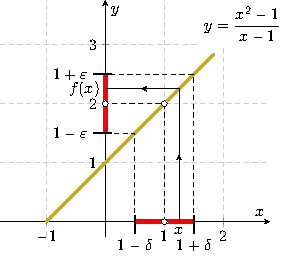
\includegraphics[width=0.45\linewidth]{mai_fig017.pdf}
   \captionof{figure}{K příkladu \ref{MAI:exam028}
   \cite[s.~118]{Brabec1989}
   \label{mai:fig017}}
  \par}
  
  Zvolíme-li libovolně malé okolí bodu \(2\), pak vždy lze najít okolí bodu \(1\) takové, že pro 
  každé \(x \neq 1\) z tohoto okolí bude ležet hodnota \(f(x)\) ve zvoleném okolí čísla \(2\). 
  Ještě jinak formulováno: K libovolně malému \(\varepsilon > 0\) existuje \(\delta > 0\) tak, 
  že pro každé \(x\), pro něž \(0 < \abs{x — 1} \ll \delta\), platí \(\abs{f(x) — 2} < 
  \varepsilon\) (viz obr. \ref{mai:fig017}). O funkci \(f\) s touto vlastností říkáme, že má v bodě 
  \(1\) limitu \(2\) a píšeme symbolicky \(lim_{x \to 1}f(x) = 2\) nebo \(f(x) \rightarrow 2\) pro 
  \(x \rightarrow 1\).
\end{example}
















    %-------------------------------------

    Definičním oborem funkce z příkladu \ref{mai:exam028} je tedy množina \(\mathcal{D} = \realset -
    {1}\) (pro \(a = 1\) by ve jmenovateli zlomku byla nula). Grafem funkce je tedy přímka s
    „vynechaným“ bodem \([1, 2]\) (obr. \ref{mai:fig017}). V bodě \(a = 1\) funkční hodnota není
    definována. Pokud bychom chtěli rozšířit definiční obor funkce na celou reálnou osu, musíme
    předepsat, jaké hodnoty má funkce nabývat v bodě \(a = 1\). Původní vzorec, jímž je funkce
    zadána, výpočet hodnoty \(f(1)\) neumožňuje. Dodatečné zadání funkční hodnoty, její
    \emph{dodefinování}, můžeme provést zcela libovolně. Zvolme například \(f(1) = 2\). Jiná
    možnost, jak funkci dodefinovat, je například \(f(1) =-1\). Které číslo je ovšem limitou funkce
    \(f(x)\) v bodě \(a = 1\)? Je to číslo \(2\), které je v případe \(f(x) = x+1\) její funkční
    hodnotou? Nebo číslo \(-1\)? A nebo nějaká jiná hodnota? Intuice nám napovídá, že je to číslo
    \(2\). Když dvojku použijeme pro dodefinování funkce, přetržený graf se „zacelí“. Vidíme, že
    vezmeme-li dostatečně malý interval proměnné \(x\) v blízkosti bodu \(a=1\) můžeme docílit toho,
    že všechny odpovídající funkční hodnoty \(f(x)\) budou ležet tak blízko hodnotě \(2\), jak si
    předem určíme. Skutečně, zkusme docílit toho, aby hodnoty \(f(x)\) ležely v intervalu
    \((\num{1.99}, \num{2.01})\), tj.
    \begin{equation*}
      \num{1.99} < x + 1 < \num{2.01} \Rightarrow \num{0.99} < x < \num{1.01},\hfill x\neq1.
    \end{equation*}
    Podařilo se. A kdybychom interval \(I(\varepsilon) = (2 - \varepsilon, 2 + \varepsilon)\) 
    funkčních hodnot kolem \(2\) ještě zmenšili, podařilo by se opět najít (o něco menší) interval 
    kolem bodu \(a = 1\) tak, aby pro všechny hodnoty \(x\) v něm (samozřejmě s případnou výjimkou 
    hodnoty \(a =2\)) platilo \(f(x)\in I(\varepsilon)\). A takto bychom mohli \(\varepsilon\) 
    stále zmenšovat. Jak by takový postup dopadl s hodnotou \(-1\), která, jak intuitivně cítíme, 
    limitou funkce v bodě \(a = 1\) není, protože je graf funkce od bodu \([-1,0]\) dost vzdálen? 
    Vezměme třeba interval (\num{-0.5}, \num{0.5}) a hledejme hodnoty \(x\) obdobně jako v 
    předchozím případě. Požadujeme
    \begin{equation*}
      \num{-0.5} < x + 1 < \num{0.5} \Rightarrow \num{-1.5} < x < \num{-0.5}.
    \end{equation*}
    Tento interval vůbec neobsahuje bod \(a = 1\). Dostali jsme se mimo blízkost bodu \(a = 1\).

    %-------------------------------------
      % !TeX spellcheck = cs_CZ
\begin{mathexam}{Najdi limitu funkce \(\varphi(x) = \sqrt[3]{x}\) v bodě \(a = 0\) pomocí
  \eqref{mai:eq037}}{exam029} 
   
  Nechť \(\varphi(x) = \sqrt[3]{x}\), \(a = 0\). Pak \[f(x) = \dfrac{\sqrt[3]{x}}{x}\]. Pro \(x \neq
  0\) je \[f(x) = \frac{1}{\sqrt[3]{x^2}}\]. Jestliže \(x \to 0\), pak hodnoty \(f(x)\) neomezeně
  vzrůstají, protože jmenovatel zlomku se blíží kladnými hodnotami k nule a čitatel je stále roven
  \(1\) (viz obr. \ref{mai:fig018}). Místo rčení \emph{„funkce neomezeně roste“} pro \(x \to 0\)
  říkáme též ]\emph{„funkce se blíží k \(+\infty\)“} pro \(x \to 0\) a píšeme 
  \begin{equation*}
    \lim\limits_{x\to 0} f(x) = +\infty \text{ nebo } f(x)\to +\infty\text{ pro } x\to0.
  \end{equation*}
  Říkáme, že limita funkce \(f\) v bodě \(0\) je rovna \(+\infty\). 
    
  {\centering
  \captionsetup{type=figure}
%   \documentclass[11pt]{standalone}
\usepackage{xltxtra}
\usepackage[usenames,x11names]{xcolor}
\usepackage{tikz}
  \usetikzlibrary{intersections}
  \usetikzlibrary{decorations.markings}
\usepackage{pgfplots}
  \pgfplotsset{compat=newest}
  
\usepackage{amsmath}

\begin{document}
  \begin{tikzpicture}[thick,scale=0.7, 
      every node/.style={transform shape},
      ]
  
  \tikzset{->-/.style={decoration={
    markings,
    mark=at position #1 with {\arrow{stealth}}},postaction={decorate}}}
    
    \begin{axis}[
      xmin = -2.5, xmax = 2.5, ymin = 0, ymax = 3.5,  % osy
      domain = -1:3.5,
      restrict y to domain=0:3.4,
      axis equal image,
      grid = major,   % both
      grid style={line width=.1pt, draw=gray!20},
      major grid style={dashed, line width=.2pt, draw=gray!40},
      clip = true,
      clip mode=individual,
      xtick={-2,-1,1,2,3,4}, % make steps of length 0.2
      ytick={0,1,2,3,4,5}, 
      axis x line = middle,
      axis y line = middle,
      xlabel={\(x\)}, ylabel={\(y\)},
      enlarge y limits={rel=0.07},
      enlarge x limits={rel=0.07},
      ]
  
        \addplot[color=Gold3, samples=100, smooth, ultra thick, unbounded coords=jump,
                 no markers, domain = 0.1:2, name path global=func1] 
           gnuplot{1/((x^2.0)^(1/3.0))};
  
        \addplot[color=Gold3, samples=100, smooth, ultra thick, unbounded coords=jump,
                 no markers, domain = -2:-0.1, name path global=func2] 
           gnuplot{real(1/((x^2.0)^(1/3.0)))};
  
        \node [fill=white] at (rel axis cs: 0.75,0.5) {\(y=\dfrac{1}{\sqrt[3]{x^2}}\)};
  
        \path[name path=line] (-1,1.5) -- (1,1.5); 
            % Intersections points
            \path [name intersections={of=func1 and line,by={P1}}] (P1) node [] {};
  
        \path[name path=line] (-1,1.5) -- (1,1.5); 
            % Intersections points
            \path [name intersections={of=func2 and line,by={Q1}}] (Q1) node [] {};
        
        \draw[black,fill=black] (P1) circle (.3ex);
        \draw[black,fill=black] (Q1) circle (.3ex);
        \path (P1 |- 3,0) -- (P1) -- (P1 -| 0,3) node (X) {};
  
        \draw[thick,red, fill=white] ([shift=(0:1mm)]X) arc (0:180:1mm);
        \draw[->-=.5, dashed]  (P1 |- 3,-0.1)  
          node[below] {\(\delta\)} -- (P1) -- (P1 -| 0,3);
        \draw[->-=.5, dashed]  (Q1 |- -3,-0.1) 
          node[below] {\(\delta\)} -- (Q1) -- (Q1 -| 0,3);
  
        \draw[line width = 2pt, red, line cap=butt] (Q1 |- 3,0) -- (P1 |- 3,0);
        
        \path[name path=line] (-0.7,2.5) -- (0.7,2.5); 
            % Intersections points
            \path [name intersections={of=func1 and line,by={P1}}] (P1) node [] {};
            \draw[->-=.4, dashed, thin,gray] (P1 |- 3,-0.05) node[below] {\(x\)} -- (P1);
            \draw[->-=1, thin, gray] (P1) -- (P1 -| 0,3) node[left, fill=white] {\(f(x)\)};
        \draw[thick,red] (X) node[below left] {\(q\)} -- ++(0cm,2.5cm);
  
       \draw[black,fill=white] (0,0) node[below left] {\(O\)} circle (.4ex);
    \end{axis}
  \end{tikzpicture}
\end{document}
  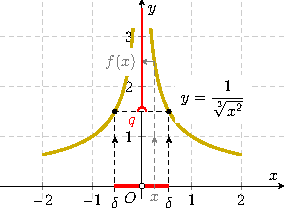
\includegraphics[width=0.8\linewidth]{mai_fig018.pdf}
  \captionof{figure}{K příkladu \ref{MAI:exam029}
  \cite[s.~118]{Brabec1989}
  \label{mai:fig018}}
  \par}
  
  Přesně to znamená toto: Zvolíme-li libovolně velké \(q > 0\), můžeme nalézt \(\delta > 0\) tak, že
  pro každé \(x \neq 0\), pro něž \(\abs{x} < \delta\), platí \(f(x) > q\). 
  
  To lze říci i takto: Zvolíme-li libovolně okolí bodu \(+\infty\), existuje okolí bodu \(0\) tak,
  že pro každé \(x \neq 0\) z tohoto okolí je \(f(x)\) ve zvoleném okolí \(+\infty\) (viz obr.
  \ref{mai:fig018}).
\end{mathexam}
















    %-------------------------------------

    Je třeba říci, že při zkoumání limit funkcí nás nezajímají jen funkce „tvaru“ 
    (\ref{mai:eq037}), i když tento případ je v diferenciálním počtu velmi častý, jak poznáme v 
    kap. \ref{mai:IchapVI}. 
    
    Někdy nás zajímá i chování funkcí v okolí nevlastních bodů \(-\infty\), \(+\infty\) 

    %-------------------------------------
      % !TeX spellcheck = cs_CZ
\begin{mdframed}[style=mdexam]
  \begin{example}\label{MAI:exam030}
    Je dána funkce \(f: f(x) = \frac{x + 1}{x}\). Sledujme její chování, když hodnoty argumentu
    \(x\) budou vzrůstat nade všechny meze neboli, jak říkáme, \(x\) se bude blížit k \(+\infty\)
    (což zapisujeme \(x \to + \infty\) (viz obr. \ref{mai:fig019}). Můžeme psát \(f(x) = 1 + 1/x\).
    Vzrůstají-li neomezeně hodnoty proměnné \(x\), blíží se hodnoty výrazu \(1/x\) čím dál tím více
    nule, takže funkční hodnoty \(f(x)\) jsou čím dál tím blíže číslu \(1\). V tomto případě píšeme
    \(lim_{x\to+\infty} f(x) = 1\) nebo \(f(x) \to 1\) pro \(x\to +\infty\) a říkáme, že funkce
    \(f\) má v bodě \(+\infty\) limitu rovnou \(1\). Přesně to znamená toto: Zvolíme-li libovolně
    malé \(\varepsilon > 0\), můžeme nalézt \(p > 0\) tak, že pro \(x > p\) platí \(\abs{f(x) - l} <
    \varepsilon\). (Viz obr. \ref{mai:fig019}.) Můžeme to říci i takto: Zvolíme-li libovolně okolí
    bodu \(1\), existuje okolí bodu \(+\infty\) tak, že pro každé \(x\) (konečné) z tohoto okolí je
    \(f(x)\) ve zvoleném okolí bodu \(1\).
    
    {\centering
    \captionsetup{type=figure}
  %   % !TeX spellcheck = cs_CZ

\documentclass[11pt]{standalone}
\usepackage{xltxtra}
\usepackage[usenames,x11names]{xcolor}
\usepackage{tikz}
  \usetikzlibrary{intersections}
  \usetikzlibrary{decorations.markings}
\usepackage{pgfplots}
  \pgfplotsset{compat=newest}
  
\usepackage{amsmath}

\begin{document}
  \begin{tikzpicture}[thick,scale=0.7, 
      every node/.style={transform shape},
      ]
  
  \tikzset{->-/.style={decoration={
    markings,
    mark=at position #1 with {\arrow{stealth}}},postaction={decorate}}}
    
    \begin{axis}[
      xmin = -0.5, xmax = 5.5, ymin = 0, ymax = 4.5,  % osy
      domain =0.2:5,
      restrict y to domain=0:4,
      axis equal image,
      grid = major,   % both
      grid style={line width=.1pt, draw=gray!20},
      major grid style={dashed, line width=.2pt, draw=gray!40},
      clip = true,
      clip mode=individual,
      xtick={1,2,3,4,5}, % make steps of length 0.2
      ytick={0,1,2,3,4}, 
      axis x line = middle,
      axis y line = middle,
      xlabel={$x$}, ylabel={$y$},
      enlarge y limits={rel=0.07},
      enlarge x limits={rel=0.07},
      ]
  
      \addplot[color=Gold3, samples=100, smooth, ultra thick, unbounded coords=jump,
               no markers, domain = 0.1:5, name path global=func1] 
         gnuplot{1+1/x};
  
      \node [fill=white] at (rel axis cs: 0.4,0.75) {\(y=\dfrac{x+1}{x}\)};
  
      \path[name path=line] (0,1.7) -- (3,1.7); 
          % Intersections points
          \path [name intersections={of=func1 and line,by={P1}}] (P1) node [] {};
      
      \draw[black,fill=black] (P1) circle (.3ex);      
      \path (P1 |- 3,-0.1) node [below, fill=white] (X) {p} -- (P1) -- (P1 -| 0,3);
  
      \draw[thick,red, fill=white] ([shift=(90:2.5mm)]X) 
           arc (270:360:1mm) node(Y) {} arc (360:450:1mm);
      \draw[thin] (P1 |- 3,-0.1) -- (P1) -- (P1 -| 0,3);
      \draw[line width = 2pt,red] (Y |- 3,0)  -- ++(3.5,0);
      
   
      \draw[line width = 1pt, black, dashed] (0,1) -- ++(5,0);
      \draw[line width = 3pt, red, line cap=butt] (0,0.3) -- (0,1.7);
      \draw [thick] (-.2, 0.3) node[left] {\(1-\varepsilon\)} -- (0.1, 0.3);
      \draw [thick] (-.2, 1.7) node[left] {\(1+\varepsilon\)} -- (0.1, 1.7 );
  
      \draw[black,fill=white] (0,1) circle (.4ex);

      \path[name path=line] (2.4,0) -- ++(0,2.5); 
          % Intersections points
          \path [name intersections={of=func1 and line,by={P1}}] (P1) node [] {};
          \draw[->-=.4, dashed, gray] (P1 |- 3,-0.05) node[below] {\(x\)} -- (P1);
          \draw[->-=1,  dashed, gray] (P1) -- (P1 -| 0,3) 
            node[left] {\small\(f(x)\)};
            
    \end{axis}
  \end{tikzpicture}
\end{document}
    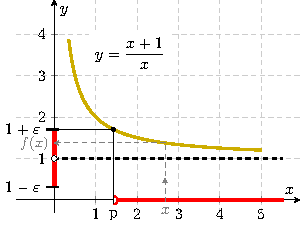
\includegraphics[width=0.45\linewidth]{mai_fig019.pdf}
    \captionof{figure}{K příkladu \ref{MAI:exam030}
    \cite[s.~119]{Brabec1989}
    \label{mai:fig019}}
    \par}
  \end{example}
\end{mdframed}
















    %-------------------------------------
    
    %-------------------------------------
      % !TeX spellcheck = cs_CZ
\begin{mdframed}[style=mdexam]
  \begin{example}\label{MAI:exam031}
    Je dána funkce \(f: f(x) = \frac{x + 1}{x}\). Sledujme její chování, když hodnoty argumentu
    \(x\) budou vzrůstat nade všechny meze neboli, jak říkáme, \(x\) se bude blížit k \(+\infty\)
    (což zapisujeme \(x \to + \infty\) (viz obr. \ref{mai:fig019}). Můžeme psát \(f(x) = 1 + 1/x\).
    Vzrůstají-li neomezeně hodnoty proměnné \(x\), blíží se hodnoty výrazu \(1/x\) čím dál tím více
    nule, takže funkční hodnoty \(f(x)\) jsou čím dál tím blíže číslu \(1\). V tomto případě píšeme
    \(lim_{x\to+\infty}f(x) = 1\) nebo \(f(x) \to 1\) pro \(x\to +\infty\) a říkáme, že funkce \(f\)
    má v bodě \(+\infty\) limitu rovnou \(1\). Přesně to znamená toto: Zvolíme-li libovolně malé
    \(\varepsilon > 0\), můžeme nalézt \(p > 0\) tak, že pro \(x > p\) platí \(\abs{f(x) - l} <
    \varepsilon\). (Viz obr. \ref{mai:fig019}.) Můžeme to říci i takto: Zvolíme-li libovolně okolí
    bodu \(1\), existuje okolí bodu \(+\infty\) tak, že pro každé \(x\) (konečné) z tohoto okolí je
    \(f(x)\) ve zvoleném okolí bodu \(1\).
    
    {\centering
    \captionsetup{type=figure}
  %   % !TeX spellcheck = cs_CZ
% xelatex -enable-write18 -shell-escape mai_fig020.tex
\documentclass[11pt]{standalone}
\usepackage{xltxtra}
\usepackage[usenames,x11names]{xcolor}
\usepackage{tikz}
  \usetikzlibrary{intersections}
  \usetikzlibrary{decorations.markings}
\usepackage{pgfplots}
  \pgfplotsset{compat=newest}
  
\usepackage{amsmath}

\begin{document}
  \begin{tikzpicture}[thick,scale=0.7, 
      every node/.style={transform shape},
      ]
  
  \tikzset{->-/.style={decoration={
    markings,
    mark=at position #1 with {\arrow{stealth}}},postaction={decorate}}}
    
    \begin{axis}[
      xmin = -2, xmax = 3.5, ymin = -2, ymax = 6,  % osy
      domain =-2:8,
      restrict y to domain=-1.5:6,
      axis equal image,
      grid = major,   % both
      grid style={line width=.1pt, draw=gray!20},
      major grid style={dashed, line width=.2pt, draw=gray!40},
      clip = true,
      clip mode=individual,
      xtick={-1,0,1,2,3,4}, % make steps of length 0.2
      ytick={-1,0,1,2,3,4,5,6,7,8}, 
      axis x line = middle,
      axis y line = middle,
      xlabel={$x$}, ylabel={$y$},
      enlarge y limits={rel=0.07},
      enlarge x limits={rel=0.07},
      ]
  
      \addplot[color=Gold3, samples=100, smooth, ultra thick, unbounded coords=jump,
               no markers, domain = -2:2, name path global=func1] 
         gnuplot{x^3};
  
      \node [fill=white] at (rel axis cs: 0.85,0.9) {\(y=x^3\)};
  
      \path[name path=line] (1.5,0) -- (1.5,6); 
          % Intersections points
          \path [name intersections={of=func1 and line,by={P1}}] (P1) node [] {};
          \draw[->-=.4, dashed, gray] (P1 |- 3,-0.05) node[below, fill=white] {\(x\)} -- (P1);
          \draw[->-=1,  dashed, gray] (P1) -- (P1 -| 0,3) 
            node[left=0.5cm, fill=white] {\small\(f(x)\)};
          \draw[dashed, gray] (P1 -| 0,3) + (-0.6cm,0cm) -- (P1 -| 0,3);
      \path[name path=line1] (0,1) -- (2,1); 
          % Intersections points
          \path [name intersections={of=func1 and line1, by={P1}}] (P1) node [] {};    
          \path (P1 |- 3,-0.1) node [below, fill=white] (X) {p} -- (P1) -- (P1 -| 0,3) 
              node[left, fill=white] (Y) {\(q\)};
  
      \draw[thick,red, fill=white] ([shift=(90:2mm)]X) 
           arc (270:360:1mm) node(x1) {} arc (360:450:1mm);
      \draw[dashed] (P1 |- 3,-0.1) -- (P1) -- (P1 -| 0,3);
      \draw[line width = 1pt,red] (x1 |- 3,0)  -- (3,0);
      
      \draw[thick,red] (0,1) -- (0,6);
      \draw[thick,red, fill=white] ([shift=(0:3.3mm)]Y) arc (0:180:1mm);;
    \end{axis}
  \end{tikzpicture}
\end{document}
    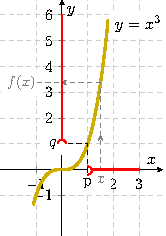
\includegraphics[width=0.35\linewidth]{mai_fig020.pdf}
    \captionof{figure}{K příkladu \ref{MAI:exam031}
    \cite[s.~119]{Brabec1989}
    \label{mai:fig020}}
    \par}
  \end{example}
\end{mdframed}
    %-------------------------------------
    
    V uvedených případech bychom mohli zkoumat i limity funkcí pro \(x \to - \infty\).  Všimněme si 
    ještě, že ve všech případech nebylo nutné, aby funkce \(f\) byla definována v bodě, ke kterému 
    se blíží hodnoty argumentu, ale bylo zapotřebí, aby funkce \(f\) byla definována v bodech 
    libovolně blízkých tomuto bodu. Tomuto požadavku bude vyhověno, jestliže daný bod, v němž 
    zkoumáme limitu, bude \emph{hromadným bodem definičního oboru}. Není ovšem nutné, aby funkce 
    byla definována v celém nějakém \emph{prstencovém okolí uvažovaného bodu}.
    
    Nechť \(a\) je bod, blízko kterého se pohybuje hodnota proměnné \(x\). Pro definici limity je 
    důležitý pojem \textbf{okolí bodu} \(a\) (obr. 2.16). Zvolme kladná čísla \(\delta_1\) a 
    \(\delta_2\). Nazýváme
    
    
  \section{Seznámení s posloupnostmi a funkcemi}\label{mai:IchapIIIsecV}  
  \section{Spojité funkce}\label{mai:IchapIIIsecVI}
  \twocolumn[\section{Derivace - rychlost změny funkce}\label{mai:IchapIIIsecVII}]
    \subsection{Hledáme tečny}\label{mai:IchapIIIsecVIIssecI}
    \subsection{Graf funkce snadno a rychle}\label{mai:IchapIIIsecVIIssecII}
    \subsection{Spokojíme se i s přibližnou hodnotou - diferenciál funkce}\label{mai:IchapIIIsecVIIssecIII}
      Pojem diferenciálu funkce \(y = f(x)\) v bodě \(a\) názorně ukazuje obrázek 2.38.
      Předpokládejme, že ke grafu funkce lze v jeho bodě \([a, f(a)]\) sestrojit tečnu. Uvažujeme o
      grafu funkce \(f(x)\) v intervalu \([a, a+h]\), kde \(h\) je \emph{přírůstek} proměnné \(x\).
      \emph{Přírůstek funkční hodnoty} neboli \emph{diference} funkce \(f(x)\) mezi body \(x = a\) a
      \(x = a+h\) je \(\Delta f = f(a+h)-f(a)\). Diferenci lze \uv{složit} sečtením přírůstku na
      tečně, který je v obrázku vyznačen symbolem \(df(a)(h)\), a hodnoty \(\chi_a(h)\), kterou lze
      považovat za funkční hodnotu jisté funkce \(\chi_a\) v bodě \(h\). Platí
      \begin{align}
        \Delta f &= f(a+h) - f(a) = df(a)(h) + \chi_a(h) =                   \nonumber      \\
                 &= h\tan\alpha+\chi_a(h) = f'(a)h + \chi_a(h)               \label{mai:eq093}
      \end{align}  
      Přírůstek na tečně, který můžeme také psát ve tvaru
      \begin{equation}\label{mai:eq094}
        df(a)(x-a) = f'(a)(x-a),
      \end{equation}
      je lineární funkcí proměnné \(h = x - a\) a nazývá se \emph{diferenciálem funkce \(f(x)\) v
      bodě \(a\)}. Pokud existuje v bodě a derivace \(f'(a)\), lze diferenciál definovat. Jaký je
      jeho význam poznáme, když prošetříme chování funkce \(\chi_a(h)\) v okolí hodnoty \(h = 0\).
      Platí

    \subsection{Poznáváme funkci z její derivace - neurčitý integrál}\label{mai:IchapIIIsecVssecIV}
    \subsection{Zpět k logaritmu a exponenciále}\label{mai:IchapIIIsecVssecV}
    \subsection{Rozmanité pohyby}\label{mai:IchapIIIsecVssecVI}
    \subsection{Od zrychlení k trajektorii}\label{mai:IchapIIIsecVssecVII}
  \twocolumn[\section{Integrování - sčítání mnoha malých příspěvků}\label{mai:IchapIIIsecVIII}]
  
%} % tikzset
%~~~~~~~~~~~~~~~~~~~~~~~~~~~~~~~~~~~~~~~~~~~~~~~~~~~~~~~~~~~~~~~~~~~~~~~~~~~~~~~~~~~~~~~~~~~~~~~~~~